%% ====================================================================
%%  Springer Nature LaTeX template  (sn-jnl.cls)  --  Nature style
%% --------------------------------------------------------------------
%%  Title: Energy sovereignty leakage: gas import substitution could
%%         relocate global emissions to mid-century
%%
%%  This file uses the official Springer Nature article template, which
%%  Nature Portfolio journals (incl. Nature Energy) accept. To compile
%%  you need the template bundle (sn-jnl.cls + sn-*.bst). Get it free:
%%    Overleaf -> "Springer Nature LaTeX Template", or
%%    https://www.springernature.com/gp/authors/campaigns/latex-author-support
%%  Place sn-jnl.cls and the .bst files next to this .tex.
%%
%%  Structure follows recent Nature Energy Articles: the opening
%%  (introduction) carries NO heading, results are presented as a run of
%%  short DECLARATIVE section headings (no "Results" parent heading),
%%  figures are embedded in the main text, and Methods follow Discussion.
%%
%%  Quantitative claims trace to the locked-model outputs (esl_results.csv,
%%  esl_results_by_regime.csv, carbon_sweep.csv); citation keys are
%%  placeholders (see the REFERENCES TO FIND checklist at end).
%% ====================================================================
%% Layout: this is ONE-COLUMN (sn-jnl default).
%% For the two-column Nature layout instead, add the iicol option:
%%   \documentclass[sn-nature,iicol]{sn-jnl}
\documentclass[sn-nature]{sn-jnl}
%% ---- packages commonly bundled with the SN template ----------------
\usepackage{graphicx}%
\usepackage{float}%   % provides [H] to pin figures exactly where cited
\usepackage{tikz}%
\usetikzlibrary{arrows.meta,positioning,shapes.geometric,fit,backgrounds}%
\usepackage{multirow}%
\usepackage{amsmath,amssymb,amsfonts}%
\usepackage{amsthm}%
\usepackage{mathrsfs}%
\usepackage[title]{appendix}%
\usepackage{xcolor}%
\usepackage{textcomp}%
\usepackage{manyfoot}%
\usepackage{booktabs}%
\usepackage{algorithm}%
\usepackage{algorithmicx}%
\usepackage{algpseudocode}%
\usepackage{listings}%
\usepackage{siunitx}%
\theoremstyle{thmstyleone}%
\newtheorem{theorem}{Theorem}%
\newtheorem{proposition}[theorem]{Proposition}%
\theoremstyle{thmstyletwo}%
\newtheorem{example}{Example}%
\newtheorem{remark}{Remark}%
\theoremstyle{thmstylethree}%
\newtheorem{definition}{Definition}%
\raggedbottom
\begin{document}
%% ---- title ---------------------------------------------------------
\title[Energy Sovereignty Leakage]{Energy sovereignty leakage: gas import
substitution could relocate global emissions to mid-century}
%% ---- authors -------------------------------------------------------
\author*[1]{\fnm{Iv\'an} \sur{Garc\'ia Kerdan}}\email{i.garciakerdan@tec.mx}
\affil[1]{\orgname{Tecnol\'ogico de Monterrey},
  \orgaddress{\city{Mexico City}, \country{Mexico}}}
%% ---- abstract & keywords ------------------------------------------
\abstract{Cutting gas imports to strengthen energy sovereignty is now explicit
policy, from Europe's retreat from Russian gas to Mexico's push for domestic
shale. Such policies are assumed to lower both dependence and global gas use. We
show this holds only conditionally, and name the failure mode \emph{Energy
Sovereignty Leakage} (ESL): the fraction of a sovereignty-driven import cut that
reappears as gas consumption elsewhere. Using a 19-region global gas-trade
model, we find ESL is not fixed but a \emph{threshold} phenomenon:
freed gas that cannot undercut the incumbent fuel abroad stays unproduced, but
once a security premium or a carbon price drives delivered liquefied natural gas
below Asian coal parity, leakage switches on. The threshold crossing is robust;
the leaked magnitude is model-dependent. Whether relocation helps or harms the
climate is contingent on upstream methane. Energy sovereignty
reshapes rather than removes global gas use.}
\keywords{energy sovereignty, carbon leakage, natural gas, LNG, methane,
energy security, global gas trade, PyPSA}
\maketitle

%% ===================================================================
%% MAIN -- opening (introduction), no heading, Nature Energy style.
%% This is the powerful, tone-setting lead of the paper. The non-specialist
%% plain-language summary has been moved to the end (submission / Editor's
%% summary field) so it does not upstage the Main.
%% ===================================================================
Natural gas sits at the intersection of two anxieties usually argued apart. One
is about carbon: gas is promoted as a lower-carbon bridge from coal yet
criticised as a fossil lock-in that commits decades of emissions \citep{Tong2019}
and whose upstream methane can erode or reverse its combustion advantage
\citep{Kemfert2022, GURSAN2021, Alvarez2018, Howarth2011, Howarth2014, Newell2014};
its net climate benefit is small when gas is cheap \citep{McJeon2014}, and rising
atmospheric methane---to which fossil sources are a leading
contributor---has sharpened the concern \citep{Saunois2020, Jackson2020}. The
other is about control: gas moves through a handful of dominant suppliers whose
reliability is now a first-order security question \citep{Bordoff2022}. Europe's
rupture with Russian gas after 2022 fused the two, elevating \emph{energy
sovereignty}---reducing import dependence through domestic supply---from rhetoric
to policy. We show the two cannot be evaluated apart: a policy chosen for
security can, under the very conditions climate policy is creating, relocate
rather than reduce global gas use.

The sovereignty premise rests on territorial reasoning: replace foreign gas
with domestic production, and both dependence and the nation's gas-related
emissions fall. But gas is globally fungible. When one country withdraws demand
from a supplier, that supplier's gas need not stay in the ground---it can be
redirected to any market willing to pay. Territorial accounting is therefore
silent on the question that decides the climate outcome: where does the
displaced gas go? This is structurally identical to \emph{carbon leakage}, in
which unilateral climate policy shifts emissions-intensive activity elsewhere
rather than eliminating it
\citep{carbonleakage, Aichele2015, FischerFox2012, Bohringer2012, Jakob2021}.
By direct analogy we define \emph{Energy Sovereignty Leakage} (ESL): the
fraction of a sovereignty-motivated cut in bilateral gas trade that is
reabsorbed as gas consumption elsewhere. An ESL of zero vindicates the
territorial framing---the world simply uses less gas; an ESL of one means the
policy merely reroutes molecules; an ESL above one, with a shift to a more
emissions-intensive supply pathway, makes it globally counterproductive.

Whether leakage occurs is not obvious, and resolving it is our central
contribution. For freed gas to \emph{add} to global consumption rather than
stay unproduced, the displaced supplier's molecules must reach a buyer at a
price that beats the incumbent fuel. We show that ESL is a \emph{threshold
phenomenon}: near zero while delivered gas sits above that competing-fuel
price, switching on once it crosses below. The mechanism is general to any
import-substitution policy; it has a sharp empirical anchor in gas re-exported
as liquefied natural gas (LNG) to Asia, where the competing fuel is coal. Two
realistic, policy-driven forces move delivered gas across this coal-parity
wall---a security premium importers pay for reliable supply, and a carbon price
that raises the cost of coal---so the instruments of the energy transition can
themselves unlock leakage. The threshold crossing is robust; the magnitude of
leakage beyond it is model-dependent, and we report it as a conditional range.

We test the mechanism on its most policy-relevant instance. Mexico is now the
world's fourth-largest gas importer, taking $\sim$68~billion cubic metres (BCM)
in 2024, almost all US pipeline gas \citep{ggr2025, eia_mexico}; successive
governments have answered this dependence with plans to develop domestic shale
\citep{sener, Alpizar2016}. That shale is a geological continuation of the plays
that made the United States the world's largest gas producer \citep{EIA_ARI2013},
yet is costlier and slower to bring online than the gas it would replace
(Fig.~\ref{fig:resourcemap})---so Mexico would pay a \emph{sovereignty premium}
to self-supply. Using a 19-region global gas-trade model solved at five-year
steps to 2045---disaggregating production by resource type, each with its own
cost and upstream methane rate, representing pipelines and LNG corridors as
capacitated links, and computing emissions on a full lifecycle basis by coupling
the dispatch to a process-level inventory (Methods)---we difference a Mexican
import-substitution counterfactual against a reference case in which Mexico keeps
importing, and trace where the freed US gas goes, what it displaces, and what it
does to global emissions. Before any counterfactual is applied, the model
reproduces the observed 2025 trade structure---the United States, Norway,
Russia, Qatar and Australia as the leading exporters and Europe and the large
Asian economies as the importers---and projects its evolution to 2045: Russian
pipeline gas pivots toward China, US and Qatari LNG grow toward Asia, and
European LNG rises as Russian supply recedes (Fig.~\ref{fig:flows}). This
calibrated, evolving system---tested out of sample against historical trade
(Supplementary Information)---is the baseline against which the sovereignty
counterfactual is differenced.

\begin{figure}[H]\centering
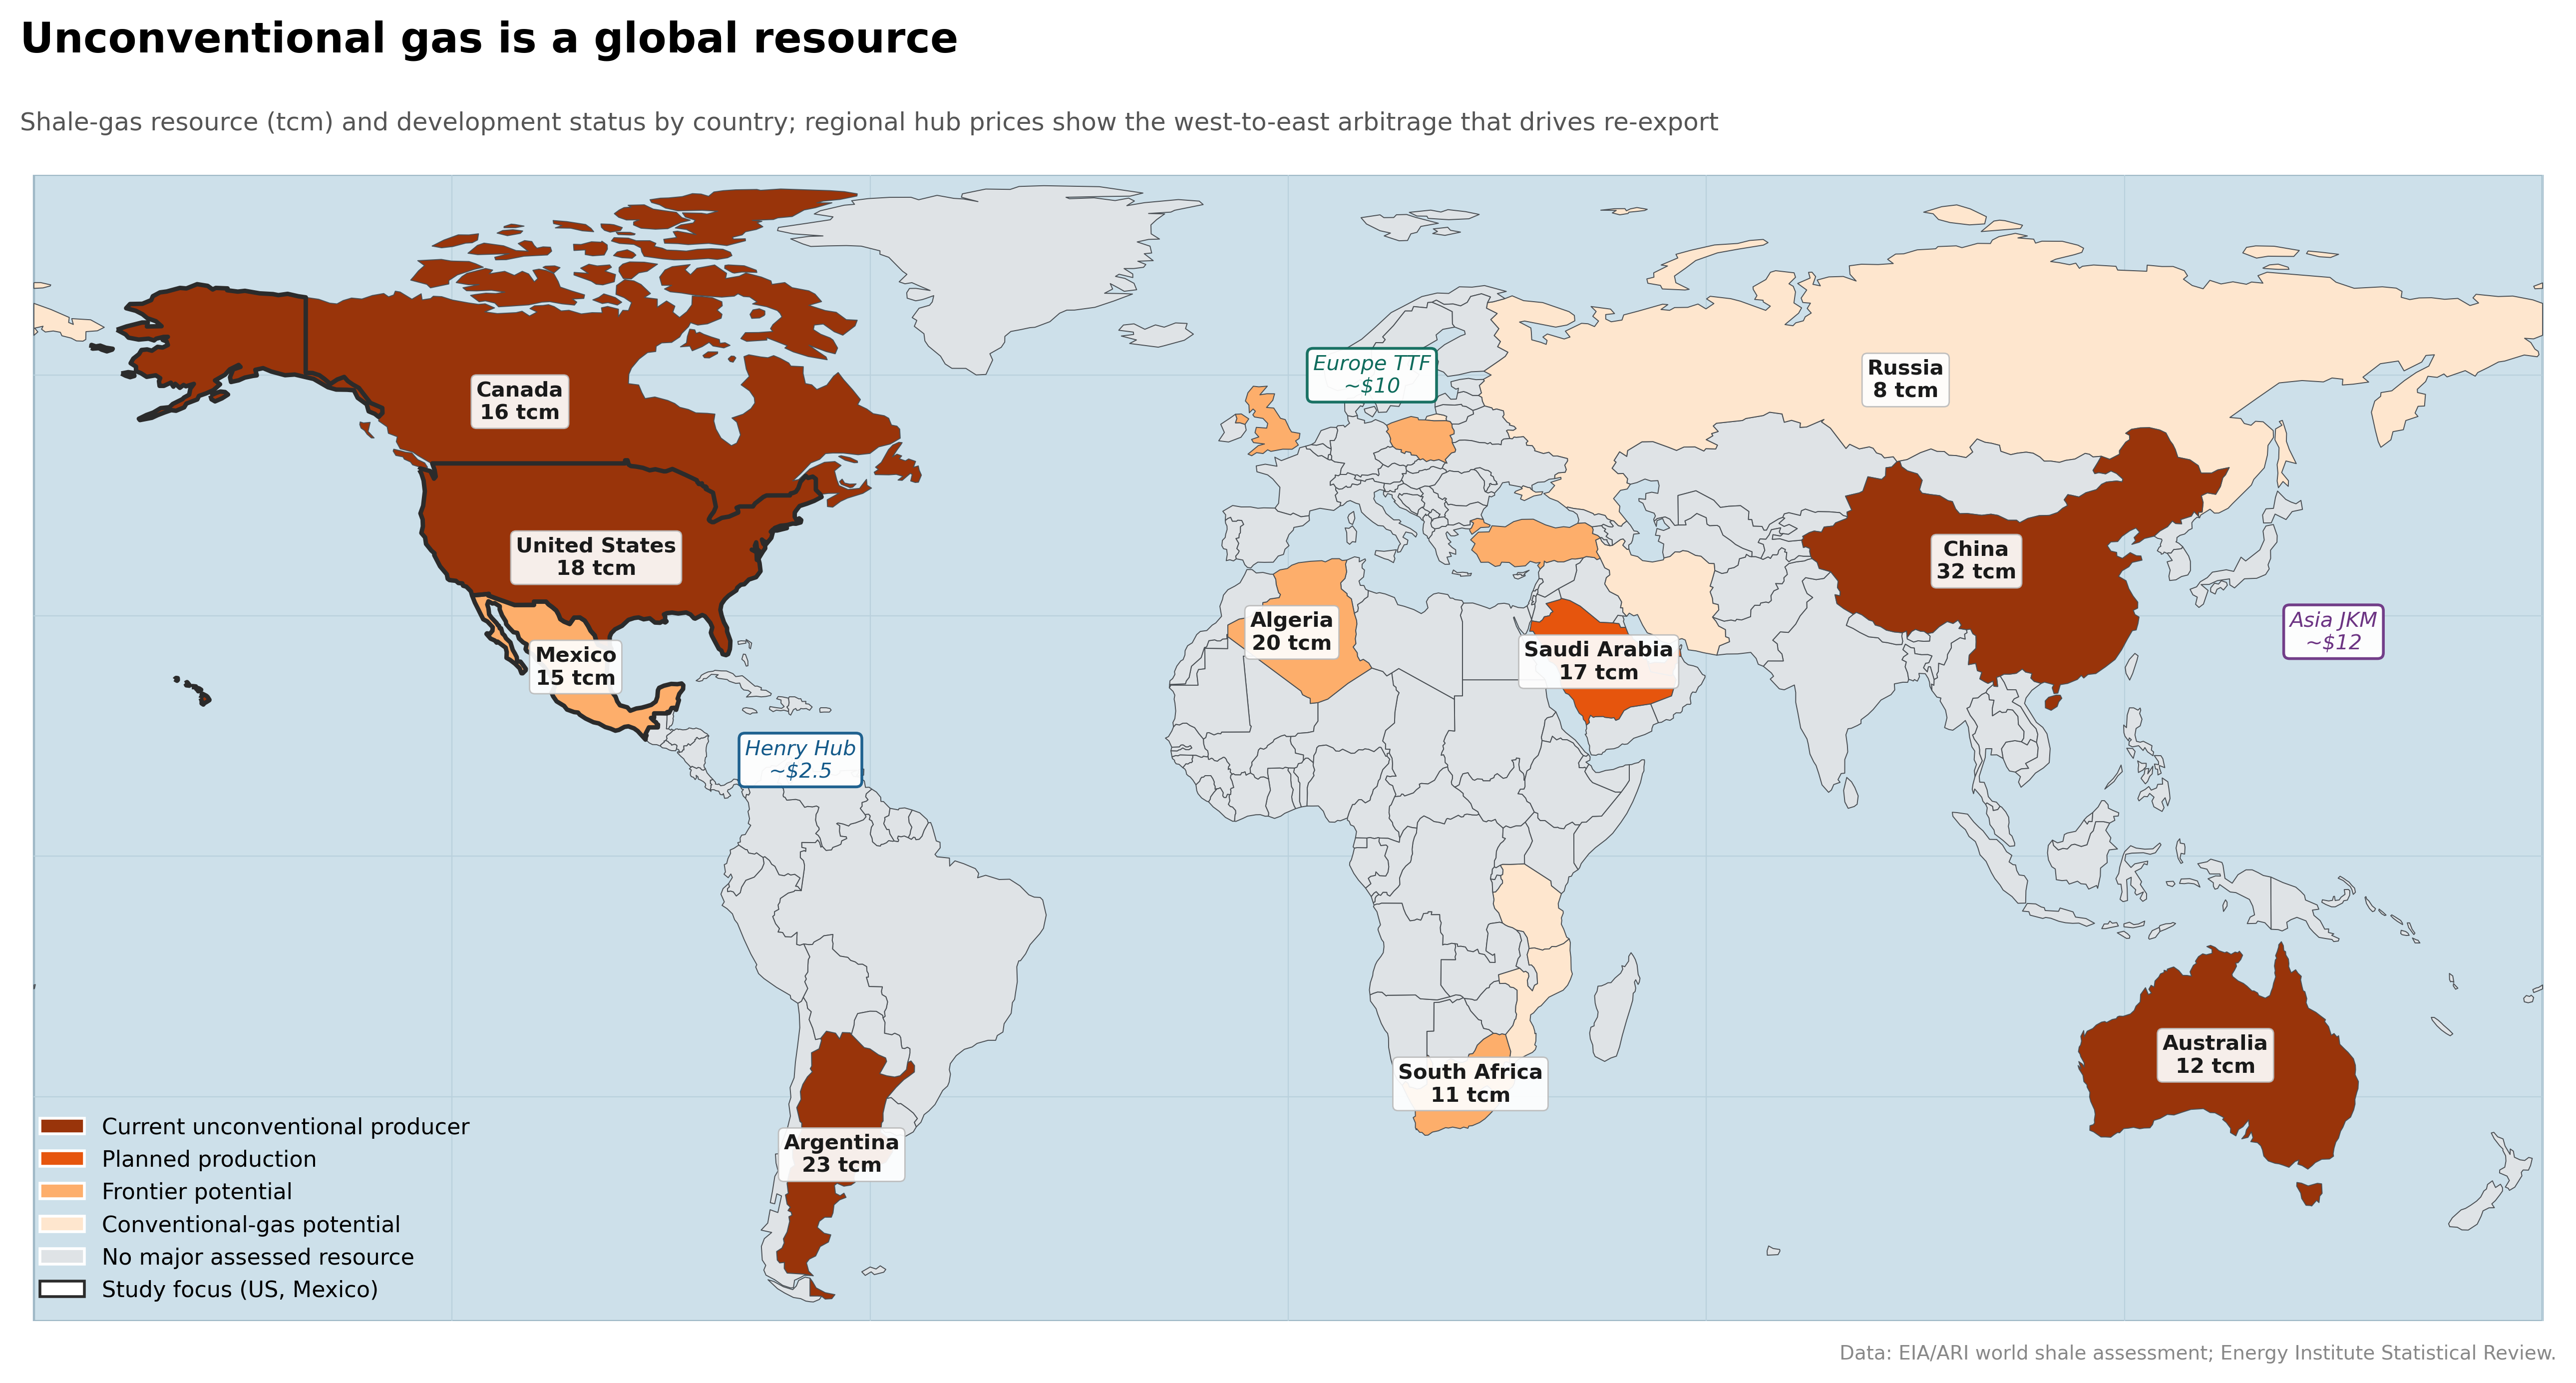
\includegraphics[width=\textwidth]{outputs/figures/Fig_unconventional_gas_map.png}
\caption{\textbf{Unconventional gas is a global resource, but unevenly
developed.} Technically-recoverable shale-gas resource (tcm) and development
status by country. Mexico (study focus) holds a large resource yet remains a
frontier producer, whereas the United States is an established, low-cost
producer---the gap that underlies the \emph{sovereignty premium} examined
here: Mexican self-supply is plausibly costlier than the US gas it would
replace. Data: EIA/ARI world shale assessment; Energy Institute Statistical
Review.}\label{fig:resourcemap}
\end{figure}

\begin{figure}[H]\centering
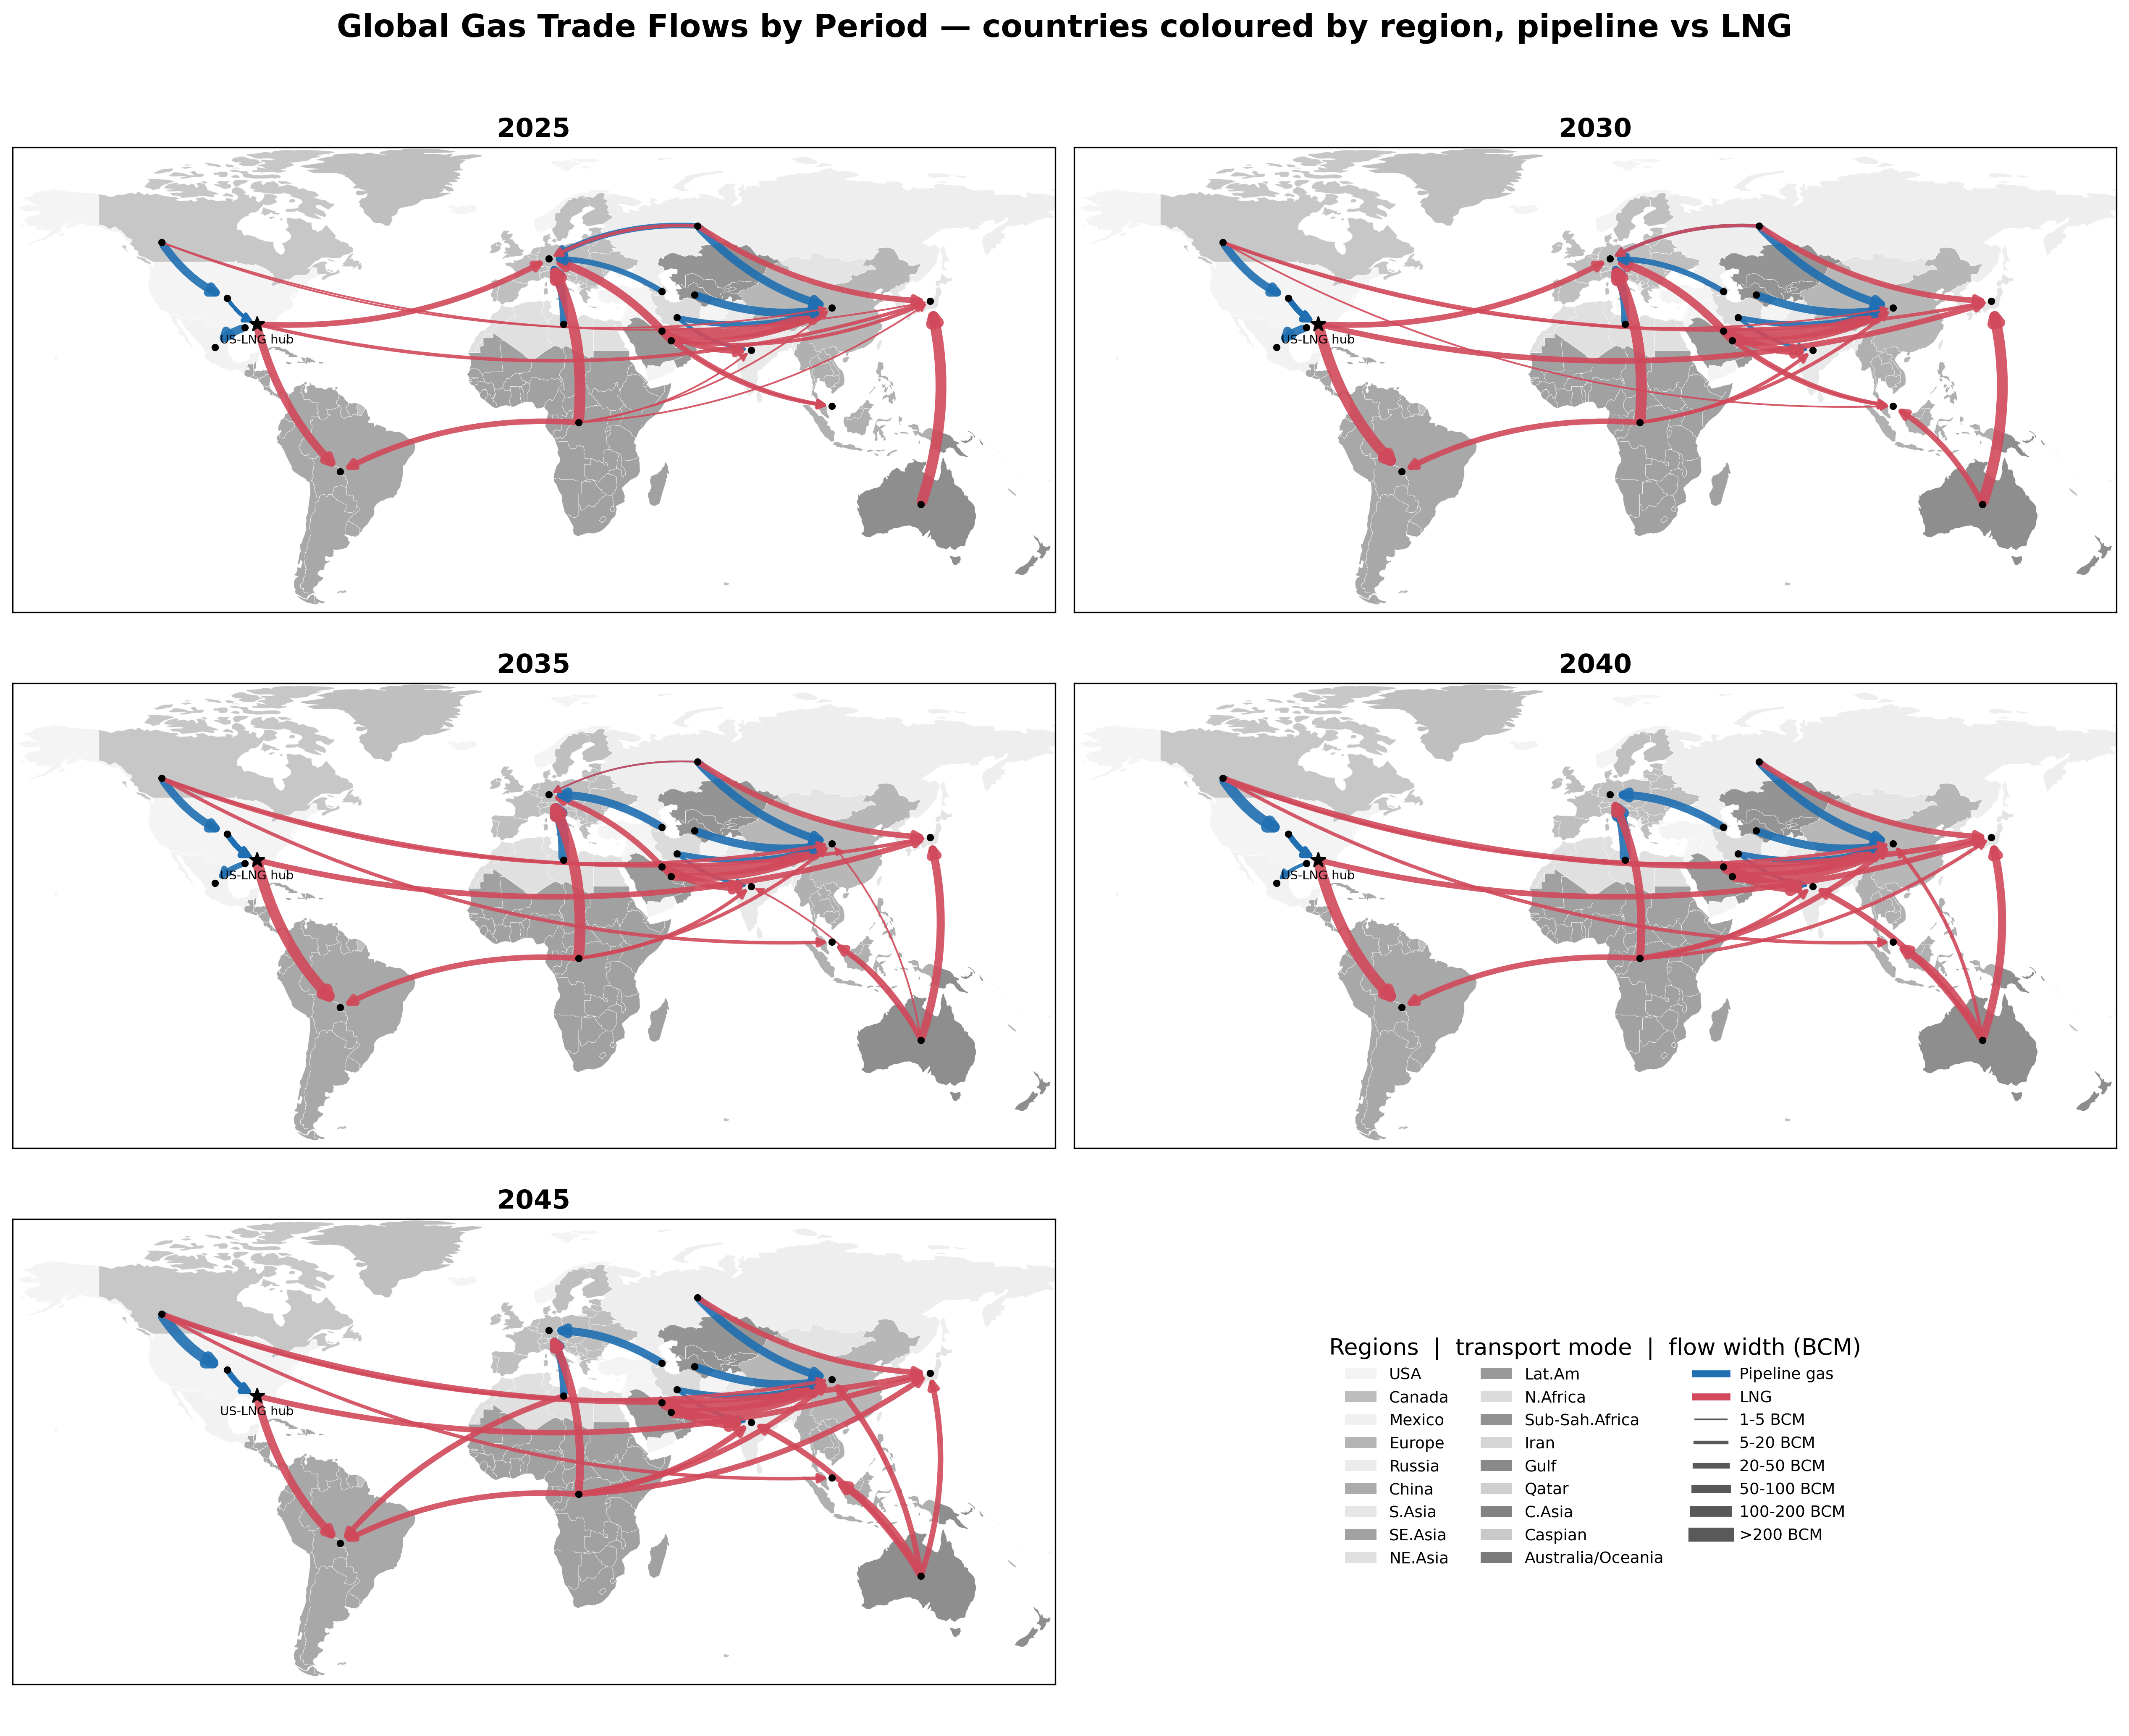
\includegraphics[width=\textwidth]{outputs/figures/WorldFlows_AllPeriods.png}
\caption{\textbf{Global gas-trade flows by period.} Modelled inter-regional gas
flows, 2025--2045, under the sovereignty case: pipeline gas (blue) and LNG
(red); countries shaded by region. The 2025 panel is the calibration baseline;
the corridors are those through which freed gas would be re-exported once the
leakage threshold is crossed.}\label{fig:flows}
\end{figure}

%% ===================================================================
%% RESULTS -- declarative section headings, no "Results" parent
%% ===================================================================
\section*{On pure economics, the freed gas is not re-exported}
In the sovereignty counterfactual Mexico develops domestic shale and phases the
US$\rightarrow$Mexico pipeline to zero; differencing against the reference case
isolates the gas Mexico's policy frees at the US Gulf---rising from negligible
levels to $\sim$66~BCM per year by 2045 (a full phase-out we take as a bounding
case: leakage scales with the freed volume, the threshold does not). The
reconfiguration is direct (Fig.~\ref{fig:naflows}): as Mexican shale ramps the
US$\rightarrow$Mexico pipeline contracts toward zero while US Gulf LNG exports
grow---but that LNG growth is almost \emph{identical} in the reference and
sovereignty cases, so the freed molecules are not re-routed into new corridors.
The per-region balance (Extended Data Fig.~2) shows the same from the demand
side: a widening US surplus, Mexico's output substituting its imports
one-for-one, and the large Asian consumers opening gaps filled by imports and
residual coal---the latent demand freed gas \emph{could} serve if it reached the
market below the price of coal. The modelled structure matches the observed 2024
market, including Mexico's rank as the fourth-largest importer \citep{ggr2025}.
We then ask how much of the freed volume reappears as gas consumption anywhere
in the world.

\begin{figure}[H]\centering
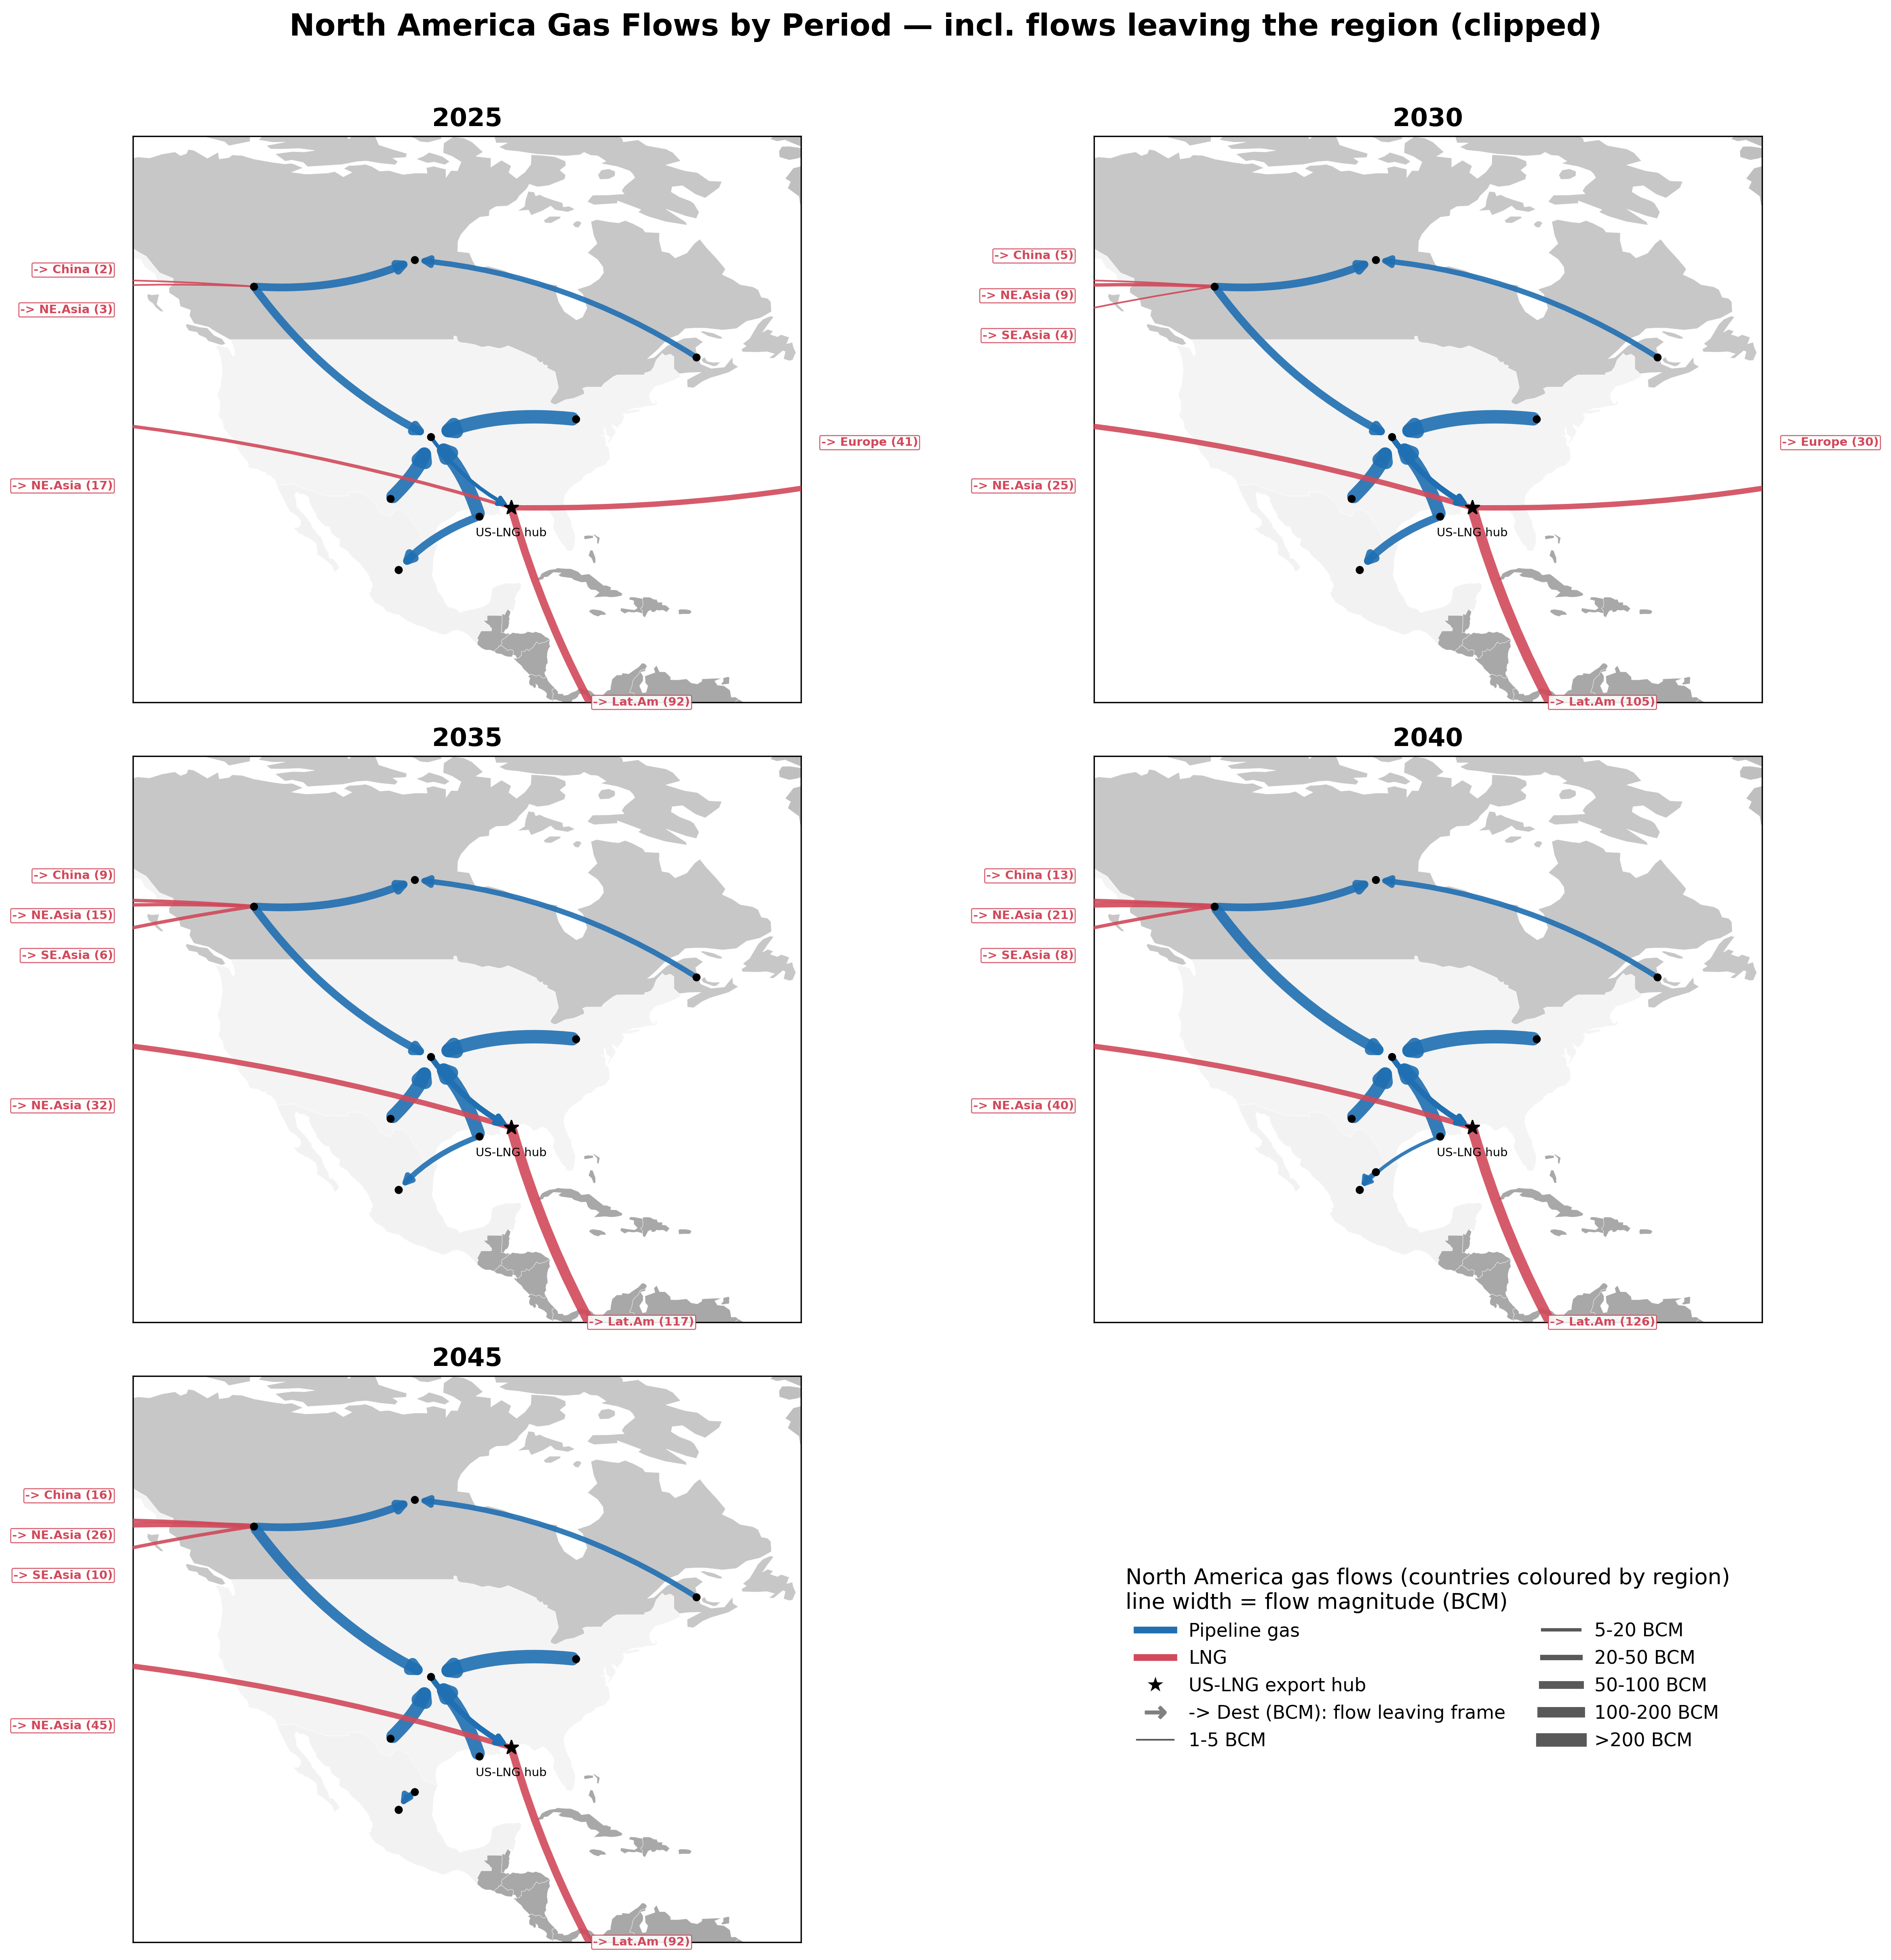
\includegraphics[width=\textwidth]{outputs/figures/NorthAmericaFlows_AllPeriods.png}
\caption{\textbf{North American gas flows by period.} Pipeline (blue) and LNG
(red) flows in and out of North America, 2025--2045, under the sovereignty case.
The US$\rightarrow$Mexico pipeline contracts as Mexican shale substitutes
imports; LNG leaving the US Gulf is the channel through which freed gas would
leak once delivered US LNG falls below coal parity.}\label{fig:naflows}
\end{figure}


Under present-day economics, almost none of it does: the central ESL is
negligible throughout ($\sim$1.7\% by 2045). The gas Mexico stops importing is,
to first order, simply \emph{not produced}---absent a profitable outlet it stays
in the ground, the outcome supply-side climate policy seeks
\citep{McGladeEkins2015, Erickson2018}---with a remainder offset by lower Mexican
demand as costlier shale raises the home price (below). This domestic response is
material: with demand held inelastic, central leakage would rise to $\sim$14\%
(Supplementary Information), so the elastic representation is the conservative
one. On economics alone, sovereignty substitution does what its proponents
intend: it lowers global gas use rather than relocating it.

The reason is a delivered-cost margin (Fig.~\ref{fig:arbitrage}). For freed US
gas to \emph{add} to consumption it must displace Asian coal, which requires US
gas---liquefied and shipped---to undercut the local coal-parity price. A
Henry-Hub-class feed cost ($\sim$2.3), liquefaction ($\sim$2.5) and
trans-Pacific shipping ($\sim$1.8) place delivered US LNG at $\sim$6.6 (model
\$/MMBtu-equivalent), just \emph{above} the $\sim$6.5 coal-parity wall, so the
freed molecules cannot out-compete coal and US export throughput is essentially
unchanged between cases. The constraint is price, not capacity: $\sim$270~BCM of
liquefaction is approved or under construction for 2030, and Asian spot LNG
traded at $\sim$10--15~\$/MMBtu over 2024--25 \citep{ggr2025}, well above the
wall. The margin that decides leakage is therefore narrow, and whether leakage
occurs hinges on which side of it delivered US LNG sits.

\begin{figure}[H]\centering
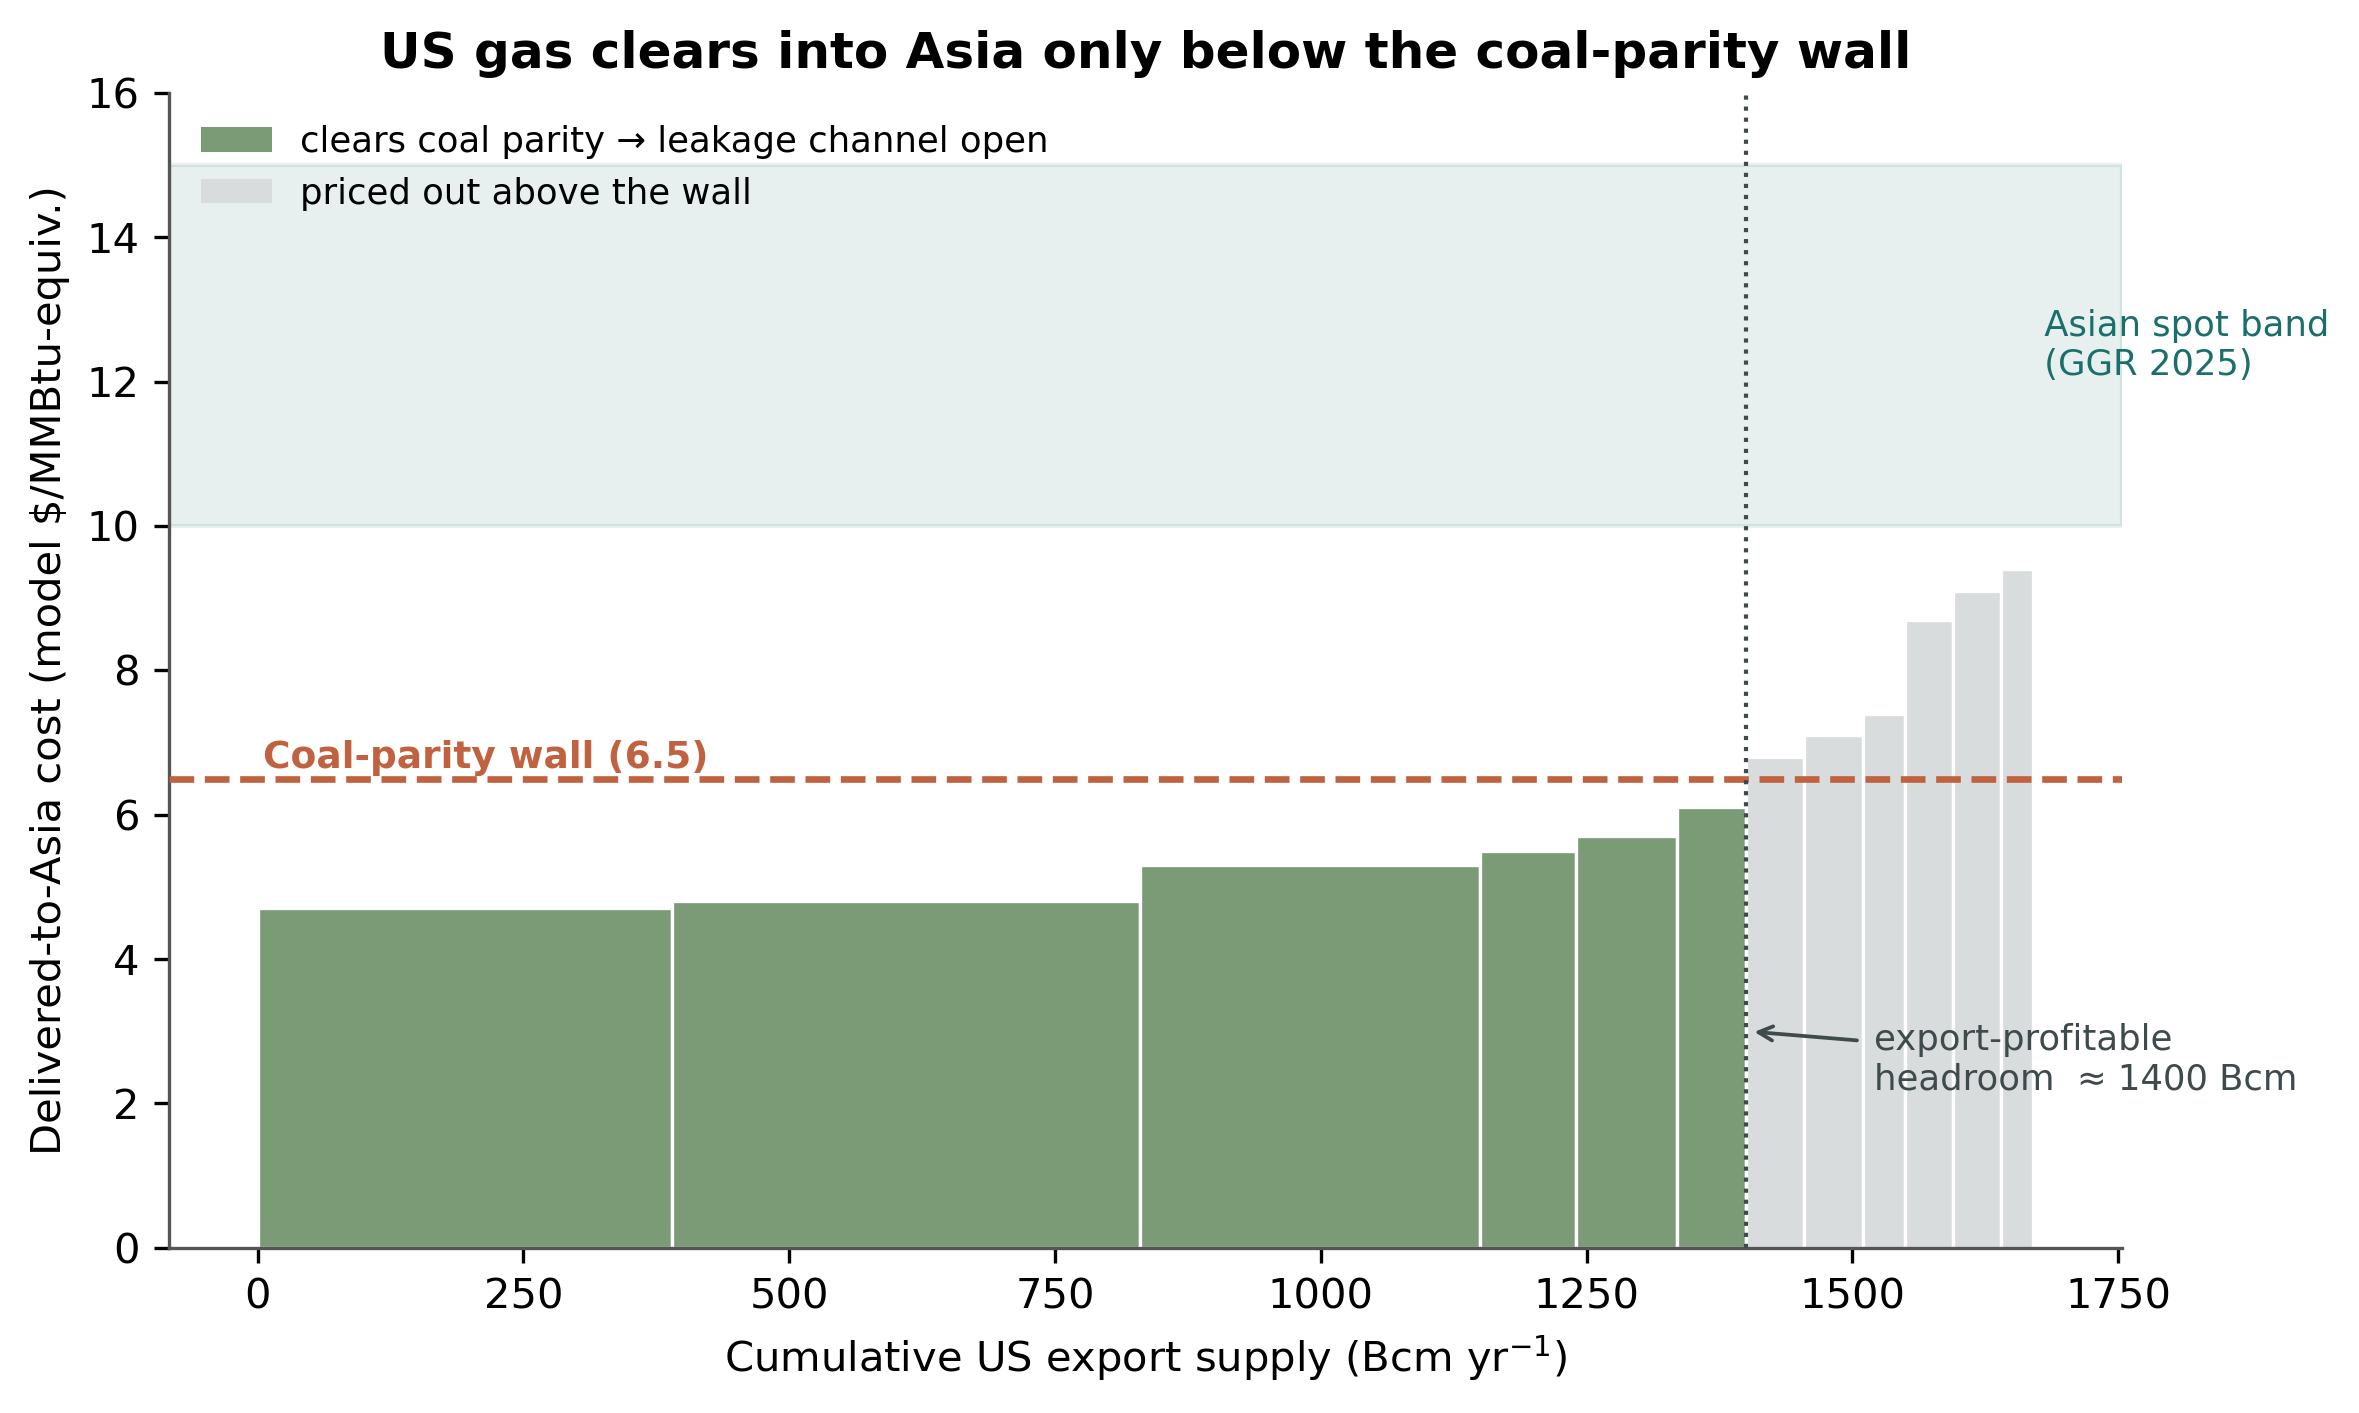
\includegraphics[width=0.92\linewidth]{outputs/figures/GGR_G1_arbitrage_merit_order.png}
\caption{\textbf{The leakage margin is a delivered-cost wall.} US gas ordered
as a delivered-to-Asia supply curve (wellhead tranche cost plus liquefaction,
capital and shipping), against the coal-parity price at which gas displaces
coal (dashed) and the observed Asian spot band \citep[shaded;][]{ggr2025}.
Tranches clearing the wall (green) open the coal-to-gas leakage channel;
higher-cost tranches (grey) are priced out. The freed Mexican volume sits near
the crossover, so small, policy-relevant shifts in the wall---a reliability
premium or a carbon price---switch leakage on.}\label{fig:arbitrage}
\end{figure}

\section*{Leakage switches on past a reliability or carbon-price threshold}
Because leakage sits just above the coal-parity wall, any force that pushes
delivered US LNG below it turns leakage on. Two are realistic and
policy-relevant, and we treat each as an explicit axis. A \emph{reliability
premium} captures buyers' willingness to pay for secure supply over
geopolitically-exposed gas---Russian supply under sanction, Gulf supply exposed
to chokepoint risk. Represented as a value that lowers the effective delivered
cost of US LNG (Methods), it leaves leakage negligible at zero but switches it
on once it exceeds $\sim$1.5~\$/MMBtu, with the mean leaked share over 2035--2045
rising into the tens of percent (Fig.~\ref{fig:threshold}a). A \emph{carbon
price} on coal does the same from the other side: $\sim$25~\$/tCO\textsubscript{2},
within the range now in force or proposed across major economies
\citep{worldbank_carbon2023, Nordhaus2015}, raises the price at which
coal-to-gas switching breaks even enough for delivered US LNG to undercut it
(Fig.~\ref{fig:threshold}b). Mechanistically the two levers act alike---both
lower delivered US LNG relative to the coal-parity wall---though the reliability
premium and US spare-capacity tightness are the cleaner levers, a carbon price
acting through the wall itself (Supplementary Information).

Two features matter. The \emph{threshold} is robust: below it leakage is
reliably near zero, and the crossing occurs where the delivered-cost arithmetic
predicts. The \emph{magnitude above it is large but conditional}---roughly
10--45\% across runs---because in a least-cost framework the leaked volume
depends on which importing markets tip from coal to gas (Methods). A global
sensitivity analysis supports this: leakage is governed by US spare export
capacity and gas cost, secondarily by coal parity and LNG-chain cost, and is
nearly insensitive to Mexican-shale cost and---for volume---to the methane rate;
on the 2035--2045 mean a 25\% leaked share is reached by tightening US spare
export capacity to $0.83\times$ central, while the reliability premium and carbon
price drive leakage into the low tens of percent without crossing 25\% across the
swept ranges (Supplementary Information). These locations are
well determined even where the magnitude is not, so we treat the threshold, not
a percentage, as the result---and its invariance to Mexican-shale cost confirms
the sovereignty premium falls on Mexico (below) rather than driving the global
leak.

\begin{figure}[H]\centering
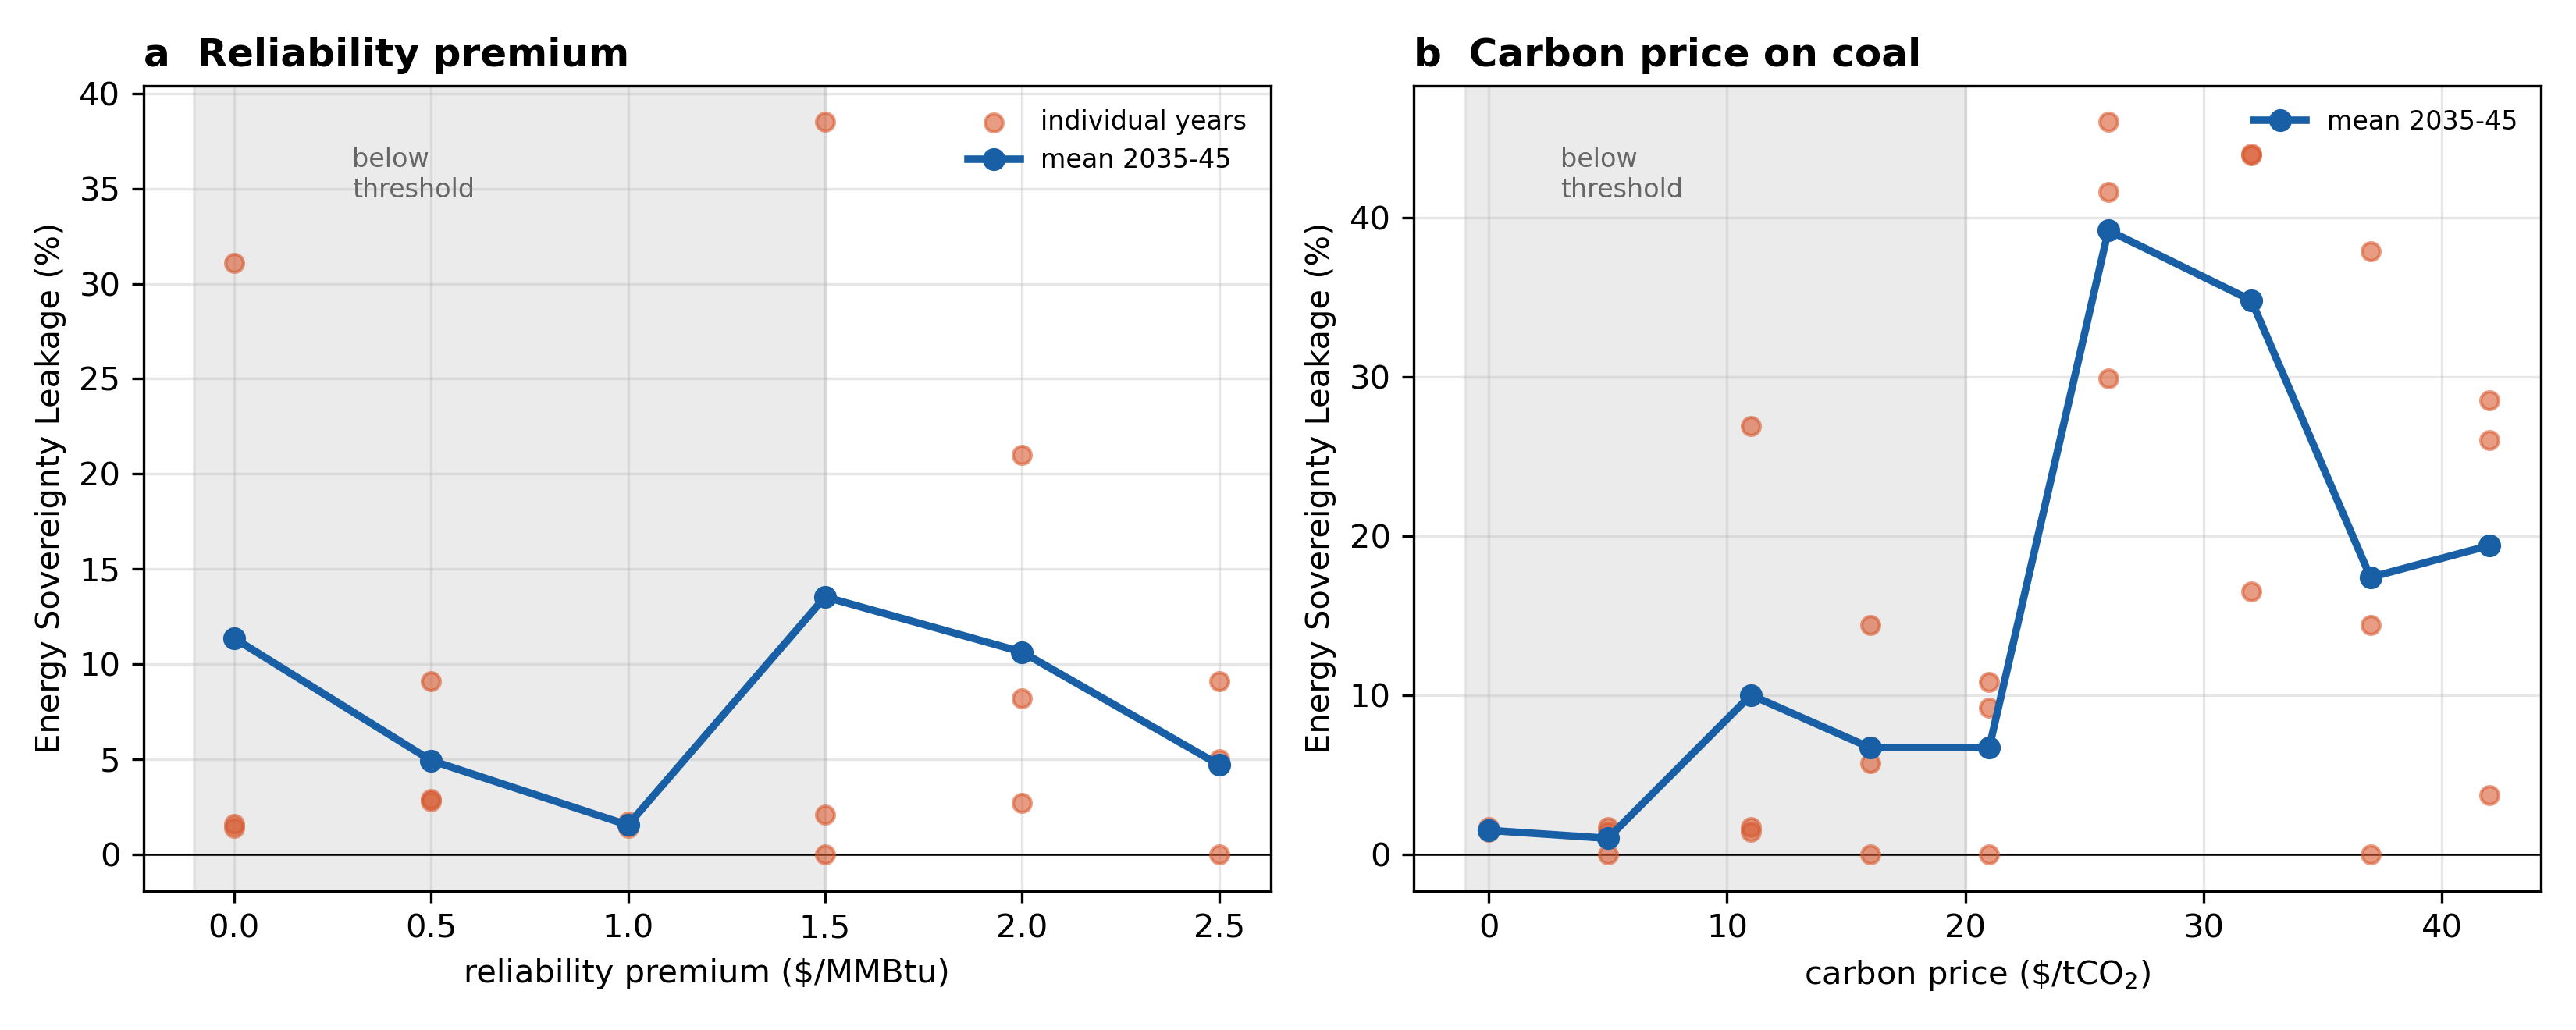
\includegraphics[width=\linewidth]{outputs/figures/ESL_thresholds.png}
\caption{\textbf{Leakage is a threshold phenomenon governed by the
delivered-US-LNG-versus-coal margin.} Energy Sovereignty Leakage (\% of the
freed bilateral volume) as a function of (\textbf{a}) the reliability premium
importers pay for secure US supply and (\textbf{b}) a carbon price on coal.
Points are individual years 2035--2045; the line is their mean. Below the
threshold (premium $\lesssim$1.5~\$/MMBtu; carbon price
$\lesssim$25~\$/tCO\textsubscript{2}) leakage is reliably near zero---freed US
gas cannot undercut coal and is left unproduced. Above it, leakage switches on
and becomes large (tens of percent) but conditional: the wide year-to-year
spread reflects the discrete, market-by-market nature of coal-to-gas switching
in a least-cost framework (Methods, Limitations), so the regime---not a single
value---is the result. Leakage is invariant to the cost of Mexican shale.}
\label{fig:threshold}
\end{figure}

\section*{Coal-to-gas switching is the leakage channel}
Coal-heavy Asian importers take extra gas only when delivered gas undercuts a
coal-parity price, represented as a spread across a heterogeneous fleet rather
than a single threshold (Methods). The channel is not hypothetical: when
Henry-Hub prices fell to historic lows in 2024, US power-sector coal-to-gas
switching rose in exactly this price-responsive way \citep{ggr2025, Cui2019}.
Below the threshold it stays shut and the freed gas is left unproduced; above
it, the coal displaced abroad tracks the leaked volume---in the carbon-priced
case ($\sim$25~\$/tCO\textsubscript{2}) the United States re-exports of order
19~BCM per year of additional LNG by 2045, displacing a comparable energy
content of Asian coal and concentrating resource drawdown on the US
unconventional base (Supplementary Information). Leakage is thus an economic
substitution that operates only when delivered shale-LNG beats coal at the
margin. Whether that switch is desirable is contested: coal retirement carries
large health co-benefits \citep{Rauner2020, Grubert2020}, yet routing
methane-intensive US gas into that role has been questioned on lifecycle grounds
\citep{GilbertSovacool2017}.

\section*{The sovereignty premium falls on Mexico}
Leakage measures what happens abroad; a distinct effect falls at home. Because
domestic shale is costlier than the US gas it replaces, Mexico's marginal price
rises as the policy deepens, and the gap to the US price---the \emph{sovereignty
premium}---widens from near zero in 2025 to several units (model
\$/MMBtu-equivalent) by the late 2030s (Fig.~\ref{fig:emissions}b). The higher
price curtails Mexican demand---23--29~BCM per year priced out rather than
served---and this domestic response, not re-export, accounts for most of the
displaced volume that does \emph{not} leak abroad. Energy sovereignty is
therefore not free: Mexico pays in higher prices and lower gas use, even as the
global system barely registers the withdrawal---a robust home-borne cost, joined
by a relocation of gas abroad only once a premium or carbon price opens the
export channel.

\begin{figure}[H]\centering
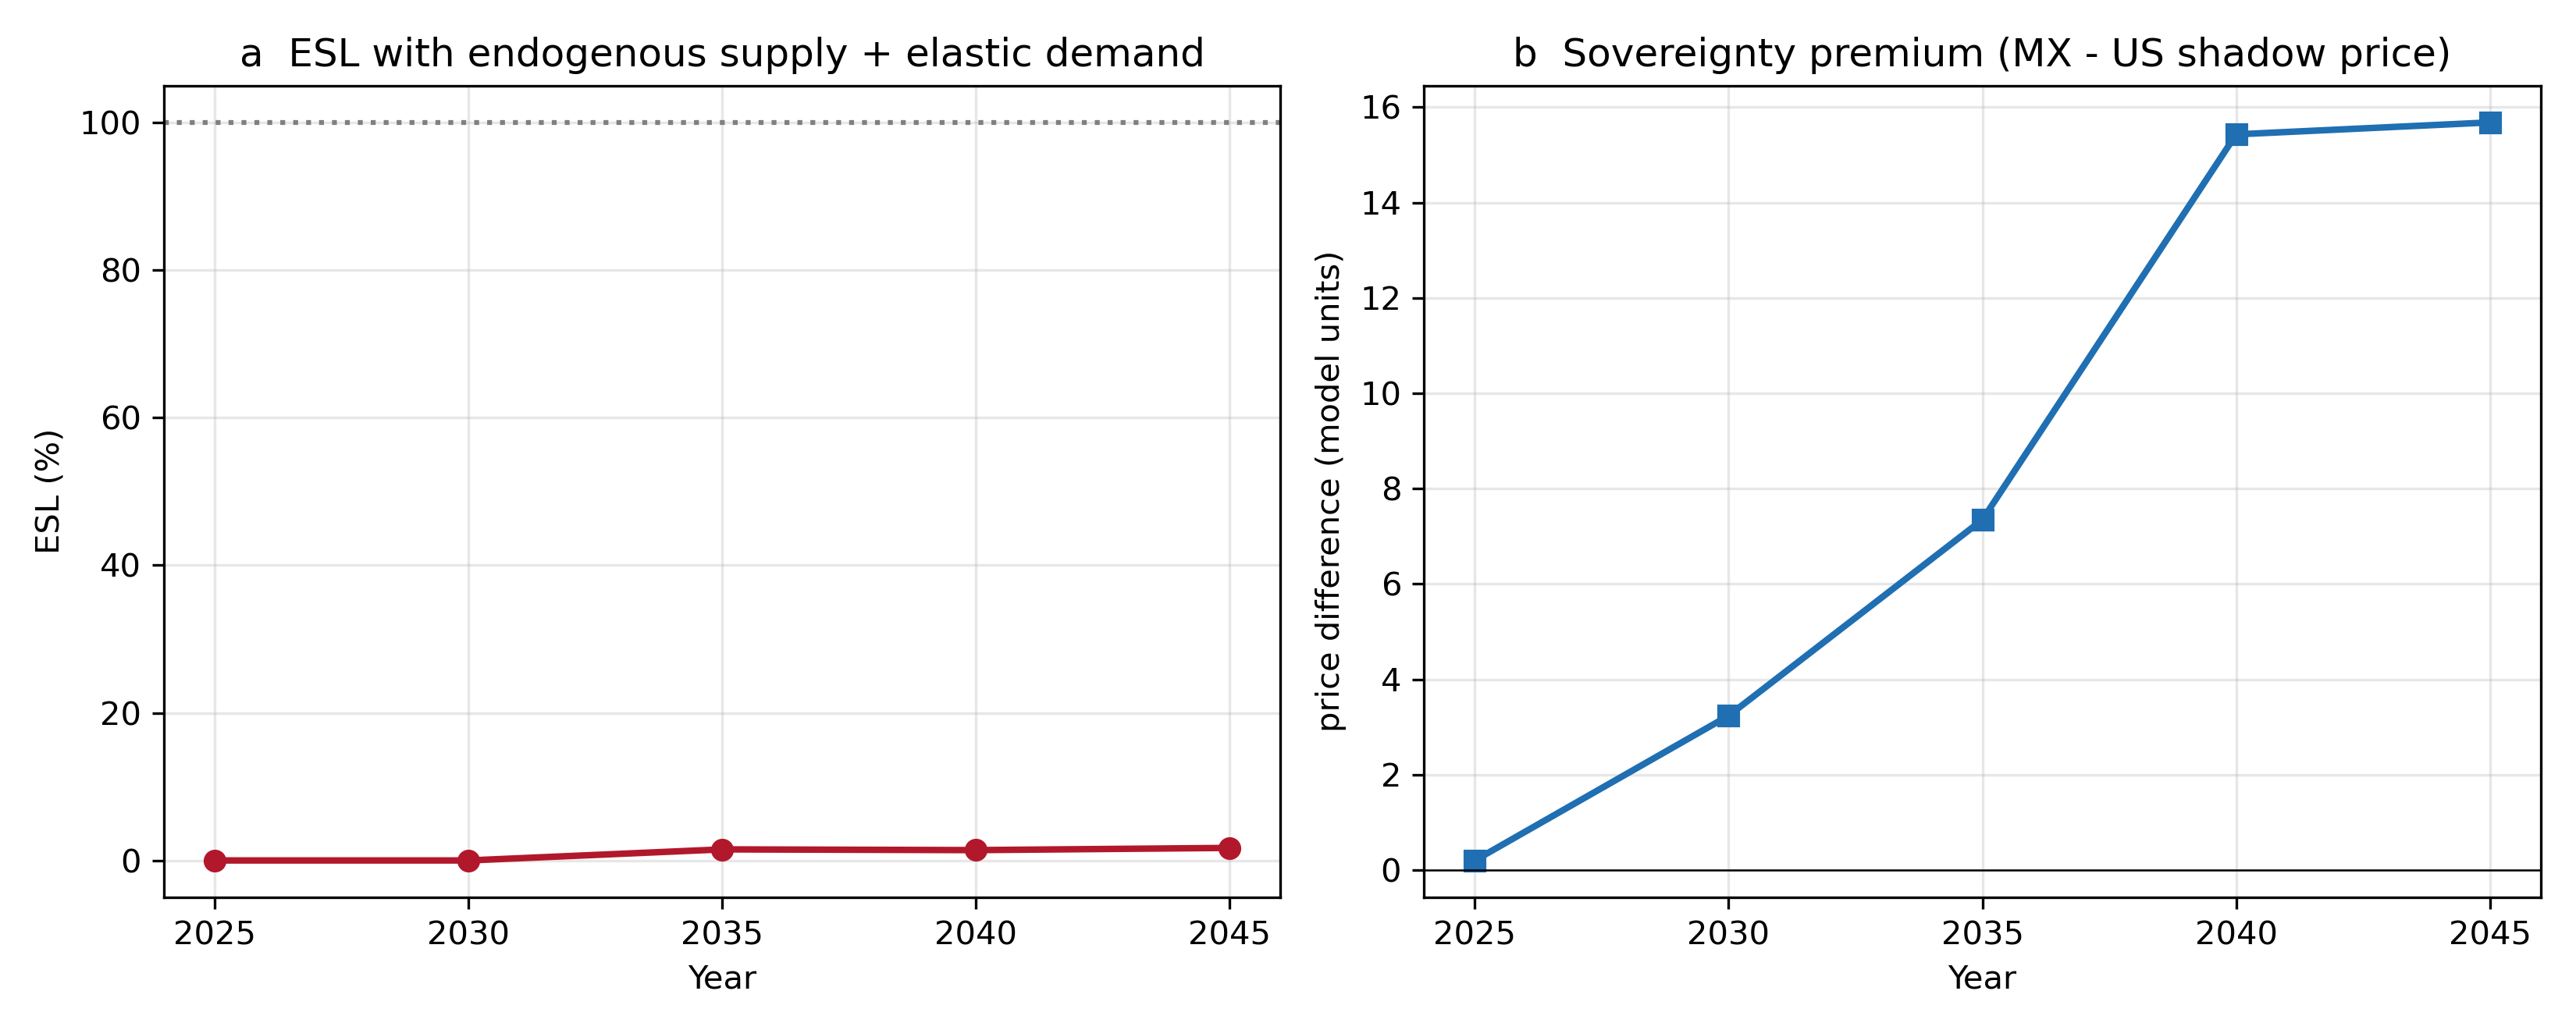
\includegraphics[width=\linewidth]{outputs/figures/ESL_improved_base.png}
\caption{\textbf{Central-case leakage and the sovereignty premium.}
\textbf{(a)} Energy Sovereignty Leakage (\%) over 2025--2045 in the central,
present-day-price calibration: negligible throughout
($\lesssim$2\%)---freed gas cannot undercut coal and is left unproduced.
\textbf{(b)} The sovereignty premium---the gap between the Mexican and US
marginal gas price---which widens as Mexico substitutes costlier domestic shale
for US imports, the cost borne by Mexico for energy sovereignty. The
associated lifecycle-emissions ledger---whose sign is methane-contingent
(leakage lowers emissions at $\sim$2.5\% methane but raises them above
$\sim$3\% under a 20-year GWP)---is reported in the text and the Supplementary
Information.}\label{fig:emissions}
\end{figure}

\section*{The climate effect of leakage is contingent on methane}
Whether coal-to-gas substitution lowers emissions turns on how the leaked
molecule---US shale gas shipped as LNG---compares with the Asian coal it
displaces over its full life cycle. We resolve this with a process-lifecycle
assessment on ecoinvent~3.9.1 in Brightway (IPCC~2021), coupled to the trade
model (Methods). The non-methane intensity is taken from ecoinvent; the upstream
methane rate, which the database carries only as a low average, is an explicit
input we vary, so the climate result is a transparent sensitivity on that rate.
Delivered US shale-LNG has an intensity of $\sim$90 and
$\sim$117~gCO\textsubscript{2}e~MJ\textsuperscript{-1} on 100- and 20-year GWP at
2.5\% methane, against $\sim$108 and $\sim$126 for coal---so at central methane
it is \emph{slightly cleaner} than coal at both horizons, consistent with
independent comparisons that find the ranking hinges on the methane rate
\citep{Gordon2023}.

The climate sign of leakage is therefore contingent, not fixed
(Fig.~\ref{fig:emissions}). Netting gas burned against coal displaced, leakage
at central methane modestly \emph{lowers} global emissions---of order
6--12~Mt~CO\textsubscript{2}e per year by 2045 in the carbon-priced regime that
switches it on (the smaller figure on a 20-year, the larger on a 100-year GWP). But shale-LNG crosses coal at $\sim$3.1\% methane on a 20-year
GWP (and $\sim$5.5\% on 100-year): in the high-methane case that recent
measurement-based and satellite studies report for US shale (up to $\sim$3.7\%)
\citep{Sherwin2024, Rutherford2021, Karion2013, Miller2013, Peischl2015, Omara2022},
and on the near-term horizon where the metric choice matters most
\citep{Allen2018, Shindell2012}, the sign reverses and leakage \emph{raises}
emissions by several Mt~CO\textsubscript{2}e per year. The climate cost is thus
real but conditional---present in the high-methane, short-horizon regime, absent
or mildly beneficial otherwise.

Crucially, the parameter that decides the sign---upstream methane---lies outside
the trade model, and is exactly where measurement-based estimates diverge most
from database averages. That divergence is resolving toward higher values as
satellite and site-level monitoring displaces inventory factors and enters LNG
contracting and regulation \citep{ggr2025}, so the term that flips the climate
outcome is the one now under active re-measurement.

Because the emissions ledger is not a fixed factor but a live coupling---every
solved year's dispatch is passed through the process-level inventory
(Methods; Extended Data Fig.~1)---the relocation of gas is also, explicitly,
a relocation of \emph{lifecycle} emissions, resolved region by region
(Fig.~\ref{fig:regemis}). Two features stand out. Mexico's lifecycle emissions
rise as it substitutes lower-intensity imports with higher-methane domestic
shale---the sovereignty premium has a carbon counterpart at home---while the
United States' rise as it becomes the swing exporter and carries its own
upstream methane with the gas it ships. And the large Asian consumers dominate
the global total whether they are served by coal or by imported gas, which is
exactly why whether the leaked molecule is cleaner or dirtier than that coal
decides the system-wide outcome. The coupling thus renders the methane
contingency not as an assumption but as a modelled, per-region result.

\begin{figure}[H]\centering
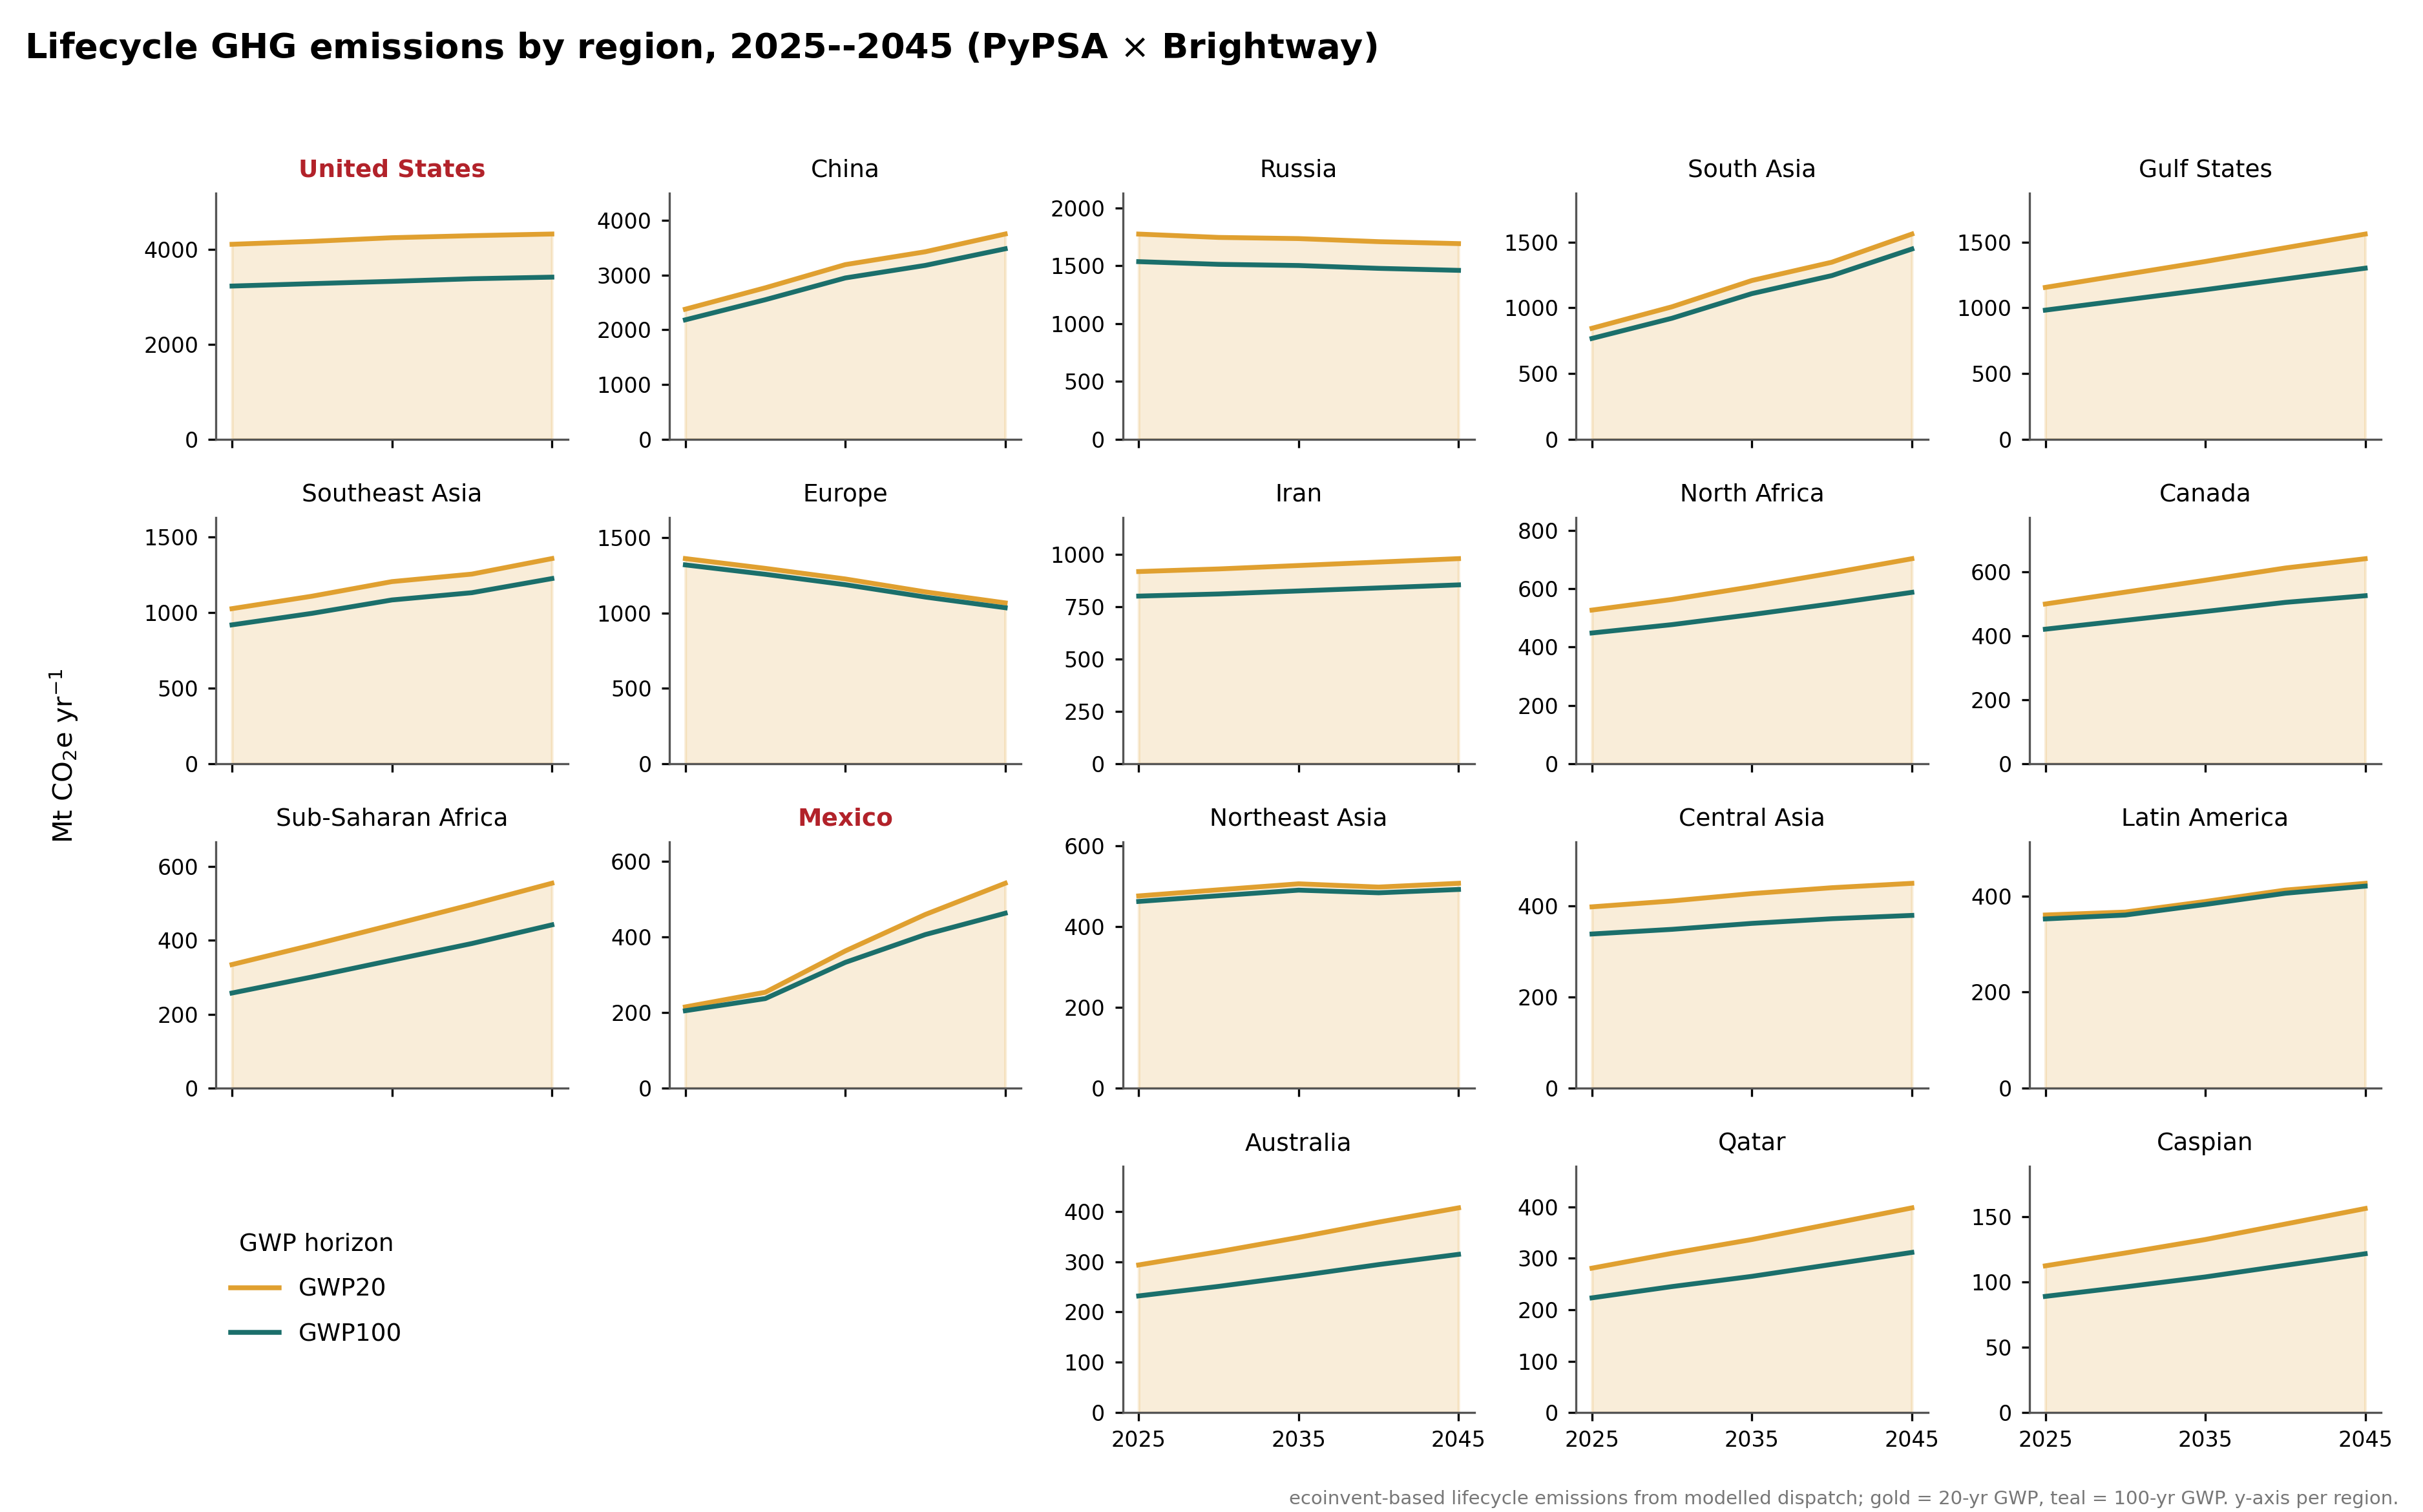
\includegraphics[width=\textwidth]{outputs/figures/Region_emissions_panels.png}
\caption{\textbf{Lifecycle greenhouse-gas emissions by region, from the
PyPSA\,$\times$\,Brightway coupling} (Mt~CO\textsubscript{2}e per year, ecoinvent
3.9.1, IPCC~2021), obtained by passing each solved year's dispatch through the
process-lifecycle inventory: 20-year GWP (gold) and 100-year GWP (teal).
Upstream methane is assigned by resource type, so US shale carries a higher
intensity than conventional or offshore gas. US and Mexican emissions rise as
each produces more shale gas, while the large Asian consumers dominate the
global total whether served by coal or imported gas. Axes are scaled per region;
United States and Mexico highlighted.}\label{fig:regemis}
\end{figure}

%% ===================================================================
\section*{Discussion}\label{sec:discussion}
Energy Sovereignty Leakage names a failure mode that territorial energy policy
cannot see. Import substitution is assumed to cut both dependence and emissions,
but in a fungible global market the displaced supplier's gas can be redirected
rather than retired. ESL measures how much is---and, like carbon leakage, the
rebound effect and the green paradox, it turns a diffuse intuition into a
quantity that can be estimated, bounded and priced. Our central finding is that
this quantity is governed by a threshold: sovereignty substitution genuinely
reduces global gas use while the freed gas cannot profitably undercut the
incumbent fuel abroad, and relocates it once the gas can. The crossing is set by
a delivered-cost margin, and the forces that move policy across it---a security
premium for trusted supply, a carbon price on coal---are the very instruments of
the current energy transition.

This connects two literatures usually kept apart: the geopolitics of energy
security, which treats import substitution as a sovereignty good, and the
climate accounting of gas, which has documented the methane and LNG-chain
penalties that make shale gas a poor coal substitute under short horizons
\citep{howarth2024, iea_methane_2024, Balcombe2018, Ocko2021}. ESL is the
bridge. It extends the logic of carbon leakage \citep{FowlieReguant2018} and the
green paradox
\citep{greenparadox, vanderPloeg2012, Jensen2015, Harstad2012, Asheim2019} to
security-motivated policy, but with a sharper, testable structure: a threshold
that determines \emph{whether} relocation occurs, and an upstream methane rate
that determines \emph{whether it matters} for the climate. It is distinct from
carbon leakage in its trigger---demand withdrawn for security, rather than
activity displaced by asymmetric climate cost---and can arise with no climate
policy at all; the two mechanisms can even act in opposite directions.

We separate what is robust from what is model-dependent. The threshold rests on
a delivered-cost comparison rather than on solver-specific behaviour: a global
sensitivity analysis locates it in the parameters that set the coal-parity
wall---US supply, gas cost, coal parity and LNG-chain cost---and its crossing
moves predictably as we vary them (Supplementary Information). The leaked
magnitude above the threshold does not carry the same weight: in a least-cost
framework it depends on which discrete markets tip from coal to gas. When we
replace that least-cost switching rule with a smooth logit market share, the
threshold crossing is unchanged while the magnitude smooths and its
market-by-market discreteness disappears (Supplementary Information)---direct
evidence that the threshold reflects the delivered-cost comparison, not the
solver. The conceptual result---that sovereignty policy has a leakage regime,
entered under identifiable conditions---therefore travels beyond this model; the
precise percentage does not, and should not be read as a universal value.

The policy lesson is about the \emph{completeness} of carbon pricing. Leakage
turns harmful through an asymmetry: a carbon price falls on coal combustion
while the upstream methane and LNG-chain emissions of the gas that displaces it
go unpriced. A lifecycle-complete price---charging the methane and LNG-chain
emissions of the competing molecule, in the spirit of border carbon adjustments
for trade-exposed goods \citep{Branger2014}---would internalise exactly the term
that decides the outcome, removing both the ambiguity and, at high methane, the
harm. This does not make sovereignty illegitimate; energy security is a
defensible objective. But sovereignty policy intended also as mitigation policy
must be coupled with explicit conditions: supply-side constraints on the
displaced exporter, demand-side measures that retire rather than re-fuel coal, or
methane and LNG-intensity standards that close the gas--coal gap. Absent them,
the molecules---and the warming---simply move.

Our conclusions are bounded by the model. The framework is a single-period,
perfect-foresight least-cost program; it omits intra-annual dynamics, storage,
contract rigidity, gas-network hydraulics and imperfect competition (the
least-cost solve is a competitive equilibrium), and price formation beyond the
coal-switching channel---which is why we report the threshold, not a leaked
percentage. An out-of-sample
back-cast reproduces the North Atlantic supply structure the counterfactual is
differenced on but is deliberately stylised for Asian import volumes
(Supplementary Information), so we rely on the direction and threshold of the
Asian response, not its calibrated magnitude. The most valuable extensions
follow: a representation with smooth inter-supplier substitution to resolve the
magnitude (a single-channel reduction already preserves the threshold);
empirical tracking of the upstream methane rate that decides the climate sign;
and whether the same threshold arises for other import-substitution
policies---critical minerals, refined fuels, ammonia. What we establish is not a
number but a way of seeing: energy sovereignty reshapes global energy use, and
whether it helps or harms the climate is decided outside the borders the policy
is designed to protect.

%% ===================================================================
\section*{Methods}\label{sec:methods}
\subsection*{Model structure}
We formulate global gas trade as a single-snapshot, least-cost optimisation
implemented in PyPSA \citep{pypsa, HorschPyPSAEur2018}, following established
practice for open, reproducible energy-system optimisation
\citep{Pfenninger2014, DeCarolis2017, Chang2021, Ringkjob2018}; per-generator quadratic supply costs make
it a convex quadratic program (see \emph{Supply curves and convexity} below).
Although PyPSA was developed for electricity systems, it is a general,
carrier-agnostic least-cost network-flow optimiser---cost-based supply and
demand at nodes connected by capacitated links---that has been extended to
multi-carrier and sector-coupled systems, including gas networks. The global
gas-trade problem is structurally identical, and PyPSA supplies exactly the
constructs the mechanism requires: per-generator marginal and quadratic costs,
capacitated and endogenously-sized links, and nodal dual prices that yield the
delivered gas price we compare against the coal-parity threshold. The network comprises 19
regional market nodes, whose roles and constituent countries are listed in
Supplementary Tables~S1 and~S2. Each region carries one or
more production \emph{generators} disaggregated by resource type, demand
\emph{loads}, and is connected to other regions by capacitated transport
\emph{links} representing pipelines and LNG corridors. A high-cost
\emph{slack} generator at each node guarantees feasibility and is verified
to remain unused in all solved years, confirming that demand is met by real
supply rather than slack.
\subsection*{Objective and constraints}
The optimiser minimises total system cost,
\begin{equation}
\min \; \sum_{g} c_g\, p_g \;+\; \sum_{\ell} k_\ell\, P_\ell^{\mathrm{nom}},
\end{equation}
where $p_g$ is the dispatch of generator $g$ with marginal cost $c_g$, and
$k_\ell$ is the annualised capital cost of any endogenously sized link
$\ell$ with installed capacity $P_\ell^{\mathrm{nom}}$. Dispatch is bounded
by installed capacity ($0 \le p_g \le P_g^{\mathrm{nom}}$), transport flows
by link capacity ($|f_\ell| \le P_\ell^{\mathrm{nom}}$), and each node
enforces mass balance between production, net imports, and demand.

\subsection*{Supply curves and convexity}
Three margins that govern leakage are represented as rising marginal-cost
\emph{curves} rather than single blocks. US production is a depletion-style
step supply curve by resource type. US liquefaction is a rising-cost curve of
tolling tranches (model \$/MMBtu-equivalent, $\sim$2.0--5.0) whose cumulative
capacity grows over time, so 2025 exposes only existing brownfield capacity
($\sim$150~BCM, keeping the baseline realistic) and later expansion costs
progressively more; this replaces a single endogenous US$\rightarrow$LNG link
and ensures the export response is smooth rather than an on/off capacity wall.
Coal-to-gas switching is likewise a spread of coal-parity prices (a
heterogeneous coal fleet) rather than one threshold. To remove the corner
solutions of a pure linear program---under which the leaked volume can jump
discontinuously between markets---we add a small per-generator quadratic cost,
giving each supplier a gently rising marginal cost; the objective is then
strictly convex and the optimum unique. The combined delivered cost of US LNG
into Asia (feed $+$ tolling $+$ shipping) is what is compared against the
coal-parity price, and the leakage threshold is the point at which it crosses.
\subsection*{Calibration}
Production capacities, costs, and trade-link capacities are calibrated to
2025 observations from the Energy Institute Statistical Review \citep{EI2024}
and agency data (US EIA, IEA \citep{iea_gas2019}). The baseline reproduces observed US marketed production
($\sim$1{,}100~BCM), US LNG exports ($\sim$150~BCM), Norwegian flows and the
US$\rightarrow$Mexico pipeline ($\sim$66~BCM) to within roughly 10--25\%; at
the regional resolution used, some importing-region totals (notably Chinese
imports) are matched only approximately, and we treat these as stylised. The
high-cost slack generator at each node is verified to remain unused in all
solved years, confirming demand is met by real supply. Forward trajectories
follow published supply outlooks rebased to the 2025 baseline. Calibration
sources and assumptions are documented in the repository
(\texttt{CALIBRATION\_NOTES.md}).
\subsection*{The sovereignty counterfactual}
We define two scenarios. In the \emph{reference} case, Mexico continues to
import US gas (US$\rightarrow$Mexico pipeline held at its 2024 level,
negligible Mexican shale). In the \emph{sovereignty} case, Mexican domestic
shale capacity ramps along a policy trajectory while the US$\rightarrow$Mexico
pipeline is phased to zero. For each year $y$ we solve both cases and compute
the displaced bilateral volume
\begin{equation}
D_y = f^{\mathrm{US}\rightarrow\mathrm{MX}}_{\mathrm{ref},y}
    - f^{\mathrm{US}\rightarrow\mathrm{MX}}_{\mathrm{sov},y},
\end{equation}
the change in total global gas consumed
$\Delta G_y = G_{\mathrm{sov},y} - G_{\mathrm{ref},y}$, and the Energy
Sovereignty Leakage ratio
\begin{equation}
\mathrm{ESL}_y = \frac{\Delta G_y}{D_y}\times 100\%.
\end{equation}
\subsection*{Reliability premium and carbon-price axes}
The conditionality of leakage is mapped along the two forces that move
delivered US LNG across the coal-parity wall. The \emph{reliability premium}
$\rho$ is a security-of-supply value (model \$/MMBtu-equivalent) that importers
assign to reliable US LNG over geopolitically-exposed supply; it is implemented
as a reduction $\rho$ in the effective delivered cost of US LNG export routes,
so that $\rho=0$ recovers pure least-cost dispatch. We sweep
$\rho \in [0, 2.5]$. The \emph{carbon price} $\tau$ (\$/tCO\textsubscript{2})
raises the cost of coal and hence the gas-coal parity price; using a coal
carbon intensity of $\sim$0.095~tCO\textsubscript{2}/MMBtu, a price $\tau$
lifts the parity threshold by $\approx 0.095\,\tau$. We sweep $\tau$ from \$0
to $\sim$\$42/tCO\textsubscript{2}. Each axis is varied around an otherwise
fixed central counterfactual, isolating the role of the
delivered-US-LNG-versus-coal margin; the two are mechanistically equivalent.
\subsection*{Coal-to-gas switching channel}
Reabsorption of freed gas is mediated by a price-responsive coal-to-gas
switching demand in coal-heavy importing regions (China, South and Southeast
Asia, Northeast Asia, with a declining European component). Each such region
carries an additional switchable load served either by gas, if delivered gas
undercuts a coal-parity price $\pi_{\mathrm{coal}}$, or by a coal-parity
backstop generator otherwise; the parity price is represented as a spread
across the fleet rather than a single value. The switchable volumes are scaled
to the regional coal fleet (\texttt{data/coal\_switch.csv}). This makes the
absorption of leaked gas an economic outcome rather than an imposed load.
\subsection*{Emissions ledger}
We attribute emissions to the leakage at the margin to avoid contamination
by least-cost re-dispatch elsewhere in the system. Lifecycle intensities of
the leaked molecule (US shale gas exported as LNG) and of the coal it displaces
are taken from a process-lifecycle assessment built on a licensed ecoinvent
3.9.1 background in Brightway, with IPCC~2021 GWP\textsubscript{100} and
GWP\textsubscript{20} characterisation and a functional unit of 1~MJ delivered
(\texttt{src/lca\_brightway.py}; Supplementary Information). We express the gas
intensity in a form that responds to the swept upstream methane-leakage rate
$r_{\mathrm{CH4}}$ (\%),
\begin{equation}
I_{\mathrm{gas}}^{(h)}(r_{\mathrm{CH4}}) = a^{(h)} + b^{(h)}\, r_{\mathrm{CH4}},
\end{equation}
where $a^{(h)}$ is the methane-independent lifecycle intensity (combustion
CO\textsubscript{2}, upstream CO\textsubscript{2}, and the
liquefaction--shipping--regasification chain) and $b^{(h)}$ the per-percent
upstream-methane contribution, evaluated on the CH\textsubscript{4}
\emph{throughput} basis (fossil CH\textsubscript{4} mass per MJ, not combustion
CO\textsubscript{2}): $a=\{74.5,\,74.5\}$ and $b=\{6.1,\,16.8\}$
gCO\textsubscript{2}e~MJ\textsuperscript{-1} for
$h=\{\mathrm{GWP}_{100},\mathrm{GWP}_{20}\}$. At the central
$r_{\mathrm{CH4}}=2.5\%$ this gives
$I_{\mathrm{gas}}=\{90,\,117\}$; the displaced coal carries
$I_{\mathrm{coal}}=\{108,\,126\}$ (combustion plus coal-mine methane, ecoinvent
3.9.1). Shale-LNG and coal break even at $r_{\mathrm{CH4}}\approx3.1\%$
(GWP\textsubscript{20}) and $\approx5.5\%$ (GWP\textsubscript{100}). The net
change is
\begin{equation}
\Delta E^{(h)}_y = \Delta G_y\, I_{\mathrm{gas}}^{(h)}
                 - C_y\, I_{\mathrm{coal}}^{(h)},
\end{equation}
where $C_y$ is the coal displaced abroad by the leaked gas. Consistent with the
marginal attribution above, we set $C_y$ to the energy-equivalent of the leaked
volume, $C_y = \Delta G_y$ (in energy terms), so that each leaked molecule is
charged against the coal it displaces one-for-one; this isolates the climate
effect of the leakage itself from the system-wide coal re-dispatch that
least-cost re-optimisation induces elsewhere. We convert from model intensity
units to mass using $1~\mathrm{BCM}$ of gas $\approx 36$~PJ, so that $1$~unit
of (gCO\textsubscript{2}e~MJ\textsuperscript{-1}~$\times$~BCM)
$=0.036$~Mt~CO\textsubscript{2}e. A stage decomposition of these lifecycle
intensities, and a note on an earlier, uncorrected methane basis, are given
in the Supplementary Information.
\subsection*{PyPSA--Brightway coupling}
Emissions are computed by coupling the trade optimisation to a process-LCA
rather than by fixed factors. Lifecycle-impact scores are linear in the
functional unit, so we evaluate a lifecycle greenhouse-gas intensity per
megajoule for each supply archetype once in Brightway (cradle-to-gate upstream
by resource type, the LNG chain, and combustion; ecoinvent~3.9.1, IPCC~2021
GWP\textsubscript{100}/GWP\textsubscript{20}) and apply these intensities to
the PyPSA dispatch of every solved year (\texttt{src/lca\_link.py}). Each
region's lifecycle emissions are assembled, without double counting, from the
upstream emissions of its production (by resource type), the combustion of its
consumption, the LNG-chain emissions of its LNG exports, and the coal it burns.
The coupling makes the model a life-cycle model---each iteration returns
per-region, per-year emissions at both horizons (Extended Data Fig.~1)---and
is consistent by construction with the marginal ledger used for the ESL climate
result (Supplementary Information).

\subsection*{Solver and reproducibility}
The program is solved with Gurobi, falling back to the open HiGHS solver;
the per-generator quadratic costs make the problem a convex quadratic program,
which both solvers handle. All inputs, scenario definitions, and the drivers
(\texttt{run\_esl.py}, \texttt{run\_carbonsweep.py}) are in the public
repository; figures are regenerated from the locked-model outputs
(Code availability).

%% ===================================================================
%% EXTENDED DATA (online-only display items; not counted among the 8 main).
%% ===================================================================
\clearpage
\section*{Extended Data}
\setcounter{figure}{0}
\renewcommand{\figurename}{Extended Data Fig.}

\begin{figure}[H]\centering
\begin{tikzpicture}[node distance=7mm and 5mm, >=Latex,
  box/.style={rectangle, rounded corners=2pt, draw=black!55, fill=blue!5,
              text width=40mm, align=center, inner sep=3.5pt, font=\scriptsize},
  data/.style={box, fill=gray!12},
  bw/.style={box, fill=teal!12, draw=teal!55},
  out/.style={box, fill=orange!14, draw=orange!60},
  arr/.style={-{Latex[length=2mm]}, thick, black!55}]
  \node[data](d1){Calibration data\\(EI Review; EIA; IEA)};
  \node[data, right=of d1](d2){Resource-type CH$_4$ rates\\(\texttt{technology.csv})};
  \node[bw, right=of d2](db){ecoinvent 3.9.1\\+ IPCC 2021 (Brightway)};
  \node[box, below=10mm of d1, xshift=18mm](build){PyPSA: build 19-region network\\(generators, links, loads)};
  \node[box, below=of build](scen){Apply scenario: reference / sovereignty;\\reliability premium $\rho$; carbon price $\tau$};
  \node[box, below=of scen](solve){Solve convex QP $\rightarrow$ dispatch:\\production, LNG flows, coal switch};
  \node[bw, right=24mm of solve](inten){Precompute lifecycle\\intensities per archetype\\(once; $I=a+b\,r$)};
  \node[box, fill=blue!9, below=of solve](couple){\textbf{Couple:} per-region lifecycle emissions\\$=$ upstream $+$ combustion $+$ LNG $+$ coal};
  \node[out, below=10mm of couple, xshift=-26mm](o1){ESL ratio\\\& threshold};
  \node[out, below=10mm of couple](o2){Per-region emissions\\(GWP$_{100}$, GWP$_{20}$)};
  \node[out, below=10mm of couple, xshift=26mm](o3){Methane-contingent\\climate result};
  \draw[arr](d1)--(build); \draw[arr](d2)--(build);
  \draw[arr](build)--(scen); \draw[arr](scen)--(solve); \draw[arr](solve)--(couple);
  \draw[arr, teal!60](db)-|(inten); \draw[arr, teal!60](inten)--(couple);
  \draw[arr, teal!60](d2.south) to[out=-90,in=90] (inten.north);
  \draw[arr](couple)--(o1); \draw[arr](couple)--(o2); \draw[arr](couple)--(o3);
\end{tikzpicture}
\caption{\textbf{Methodology and the PyPSA\,$\times$\,Brightway coupling.} The
trade optimisation (blue) is solved for each scenario and year; a process-LCA
built in Brightway on ecoinvent (teal) supplies lifecycle intensities, computed
once because impact scores are linear in the functional unit; the two are
combined into per-region lifecycle emissions and the leakage and climate results
(orange). Upstream methane enters explicitly, by resource type, from
\texttt{technology.csv}.}\label{fig:flowchart}
\end{figure}

\begin{figure}[H]\centering
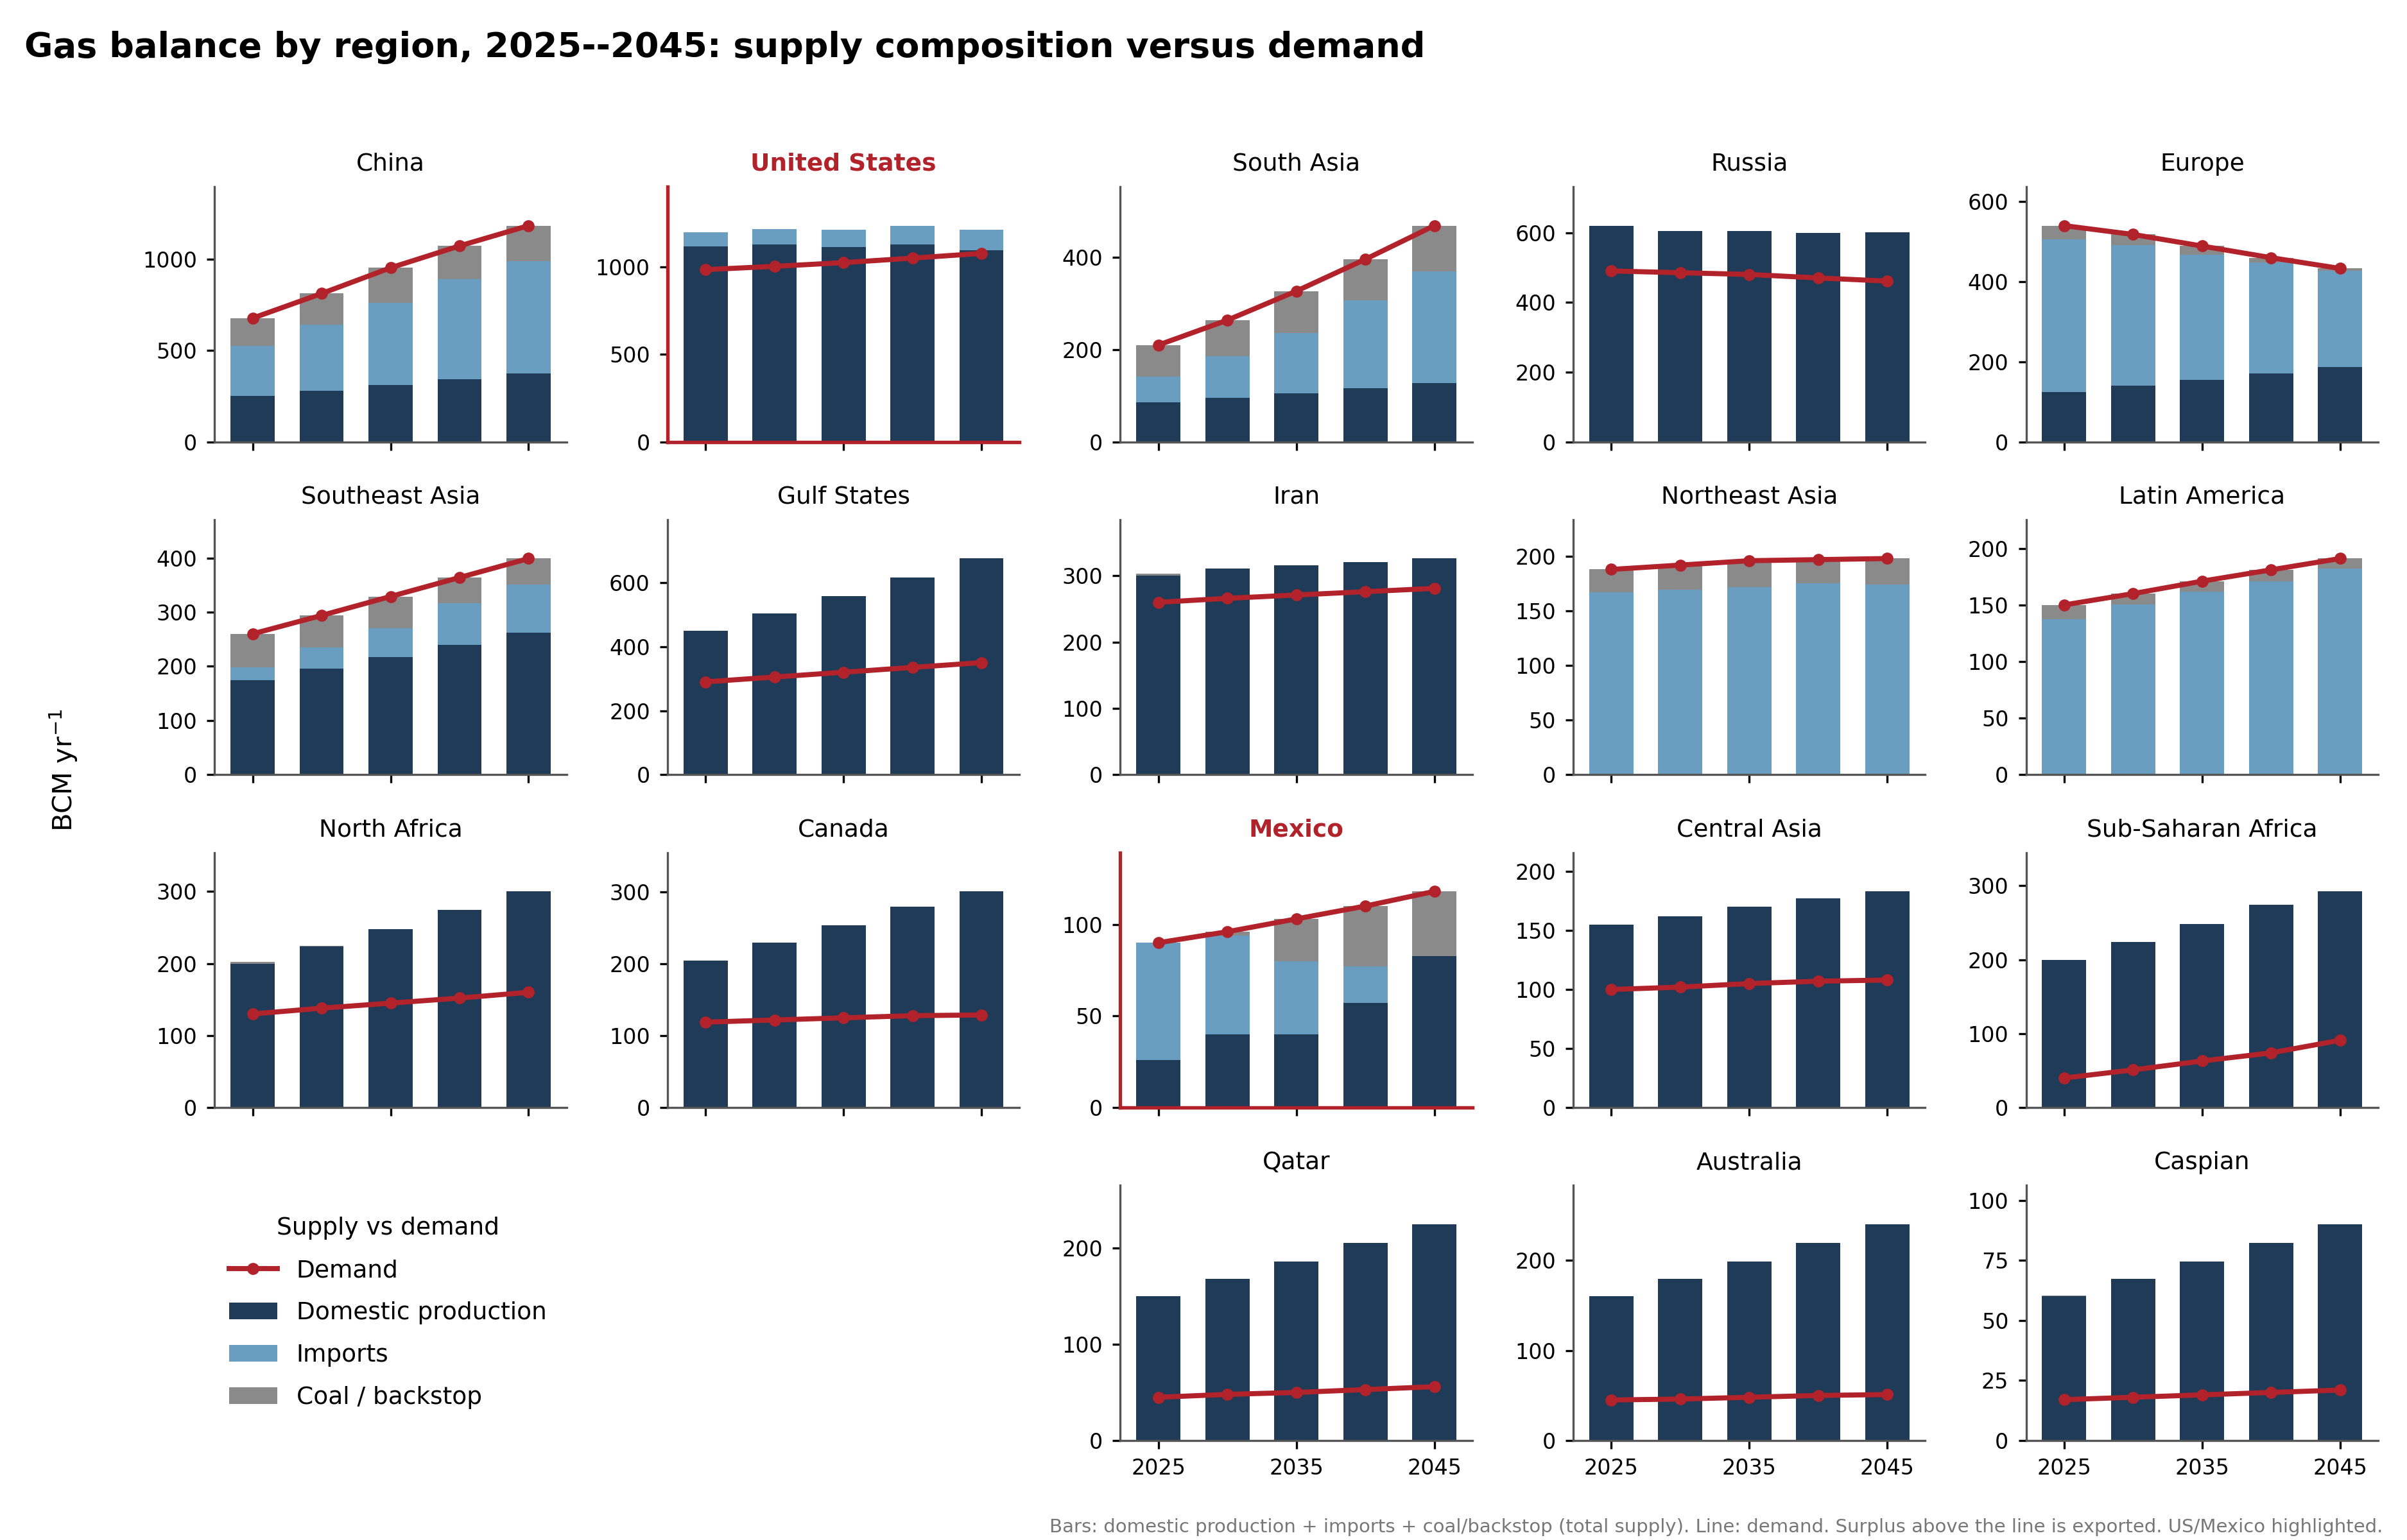
\includegraphics[width=\textwidth]{outputs/figures/Region_balance_grid.png}
\caption{\textbf{Gas balance by region, 2025--2045.} For each region, stacked
bars give supply---domestic production (navy), imports (steel) and any
coal/backstop (grey)---and the line is demand; bars above the line are exported.
The United States produces well above demand, Mexico's production rises as its
imports fall, and the large Asian consumers show widening import- and
coal-filled gaps. United States and Mexico highlighted.}\label{fig:balgrid}
\end{figure}

%% ===================================================================
\backmatter
\bmhead{Data availability}
All input data are derived from publicly available sources (Energy Institute
Statistical Review of World Energy; US Energy Information Administration;
International Energy Agency; IEA Global Methane Tracker) and are provided in
the repository. Calibration sources are documented in
\texttt{CALIBRATION\_NOTES.md}.
\bmhead{Code availability}
The PyPSA model, scenario definitions, ESL drivers, and plotting code (Python
and R) are available at [REPOSITORY URL TO ADD].
\bmhead{Author contributions}
I.G.K. designed and implemented the model and conducted the analysis and
writing.
\bmhead{Competing interests}
The author declares no competing interests.

%% ===================================================================
%%  REFERENCES TO FIND  (replace \citep keys with real citations)
%% -------------------------------------------------------------------
%%  howarth2024        Howarth (2024) - lifecycle GHG footprint of US LNG;
%%                     methane + liquefaction penalty; GWP20 vs coal.
%%  iea_methane_2024   IEA Global Methane Tracker 2024 - upstream methane
%%                     leakage rates by source/country.
%%  carbonleakage      Foundational carbon-leakage reference (e.g.
%%                     Felder & Rutherford; or IPCC AR6 WGIII synthesis).
%%  greenparadox       Green-paradox reference (Sinn 2008, "Public policies
%%                     against global warming", Int. Tax Public Finance; or
%%                     Sinn 2012, The Green Paradox, MIT Press).
%%  eia_mexico         US EIA - Mexico natural gas imports / dependence.
%%  sener              SENER / Mexican energy-sovereignty policy document.
%%  pypsa              Brown, Horsch & Schlachtberger (2018), PyPSA, JOSS.
%%  ei_statreview      Energy Institute Statistical Review of World Energy.
%%  ipcc_ar6_gwp       IPCC AR6 WGI - GWP100=30, GWP20~82.5 for fossil CH4.
%%  Kemfert2022        Kemfert et al. (2022) - gas as fossil lock-in / risk.
%%  GURSAN2021         Gursan & de Gooyert (2021) - role of gas in transition.
%% -------------------------------------------------------------------
\bibliography{sn-bibliography}   %% add references.bib, keep sn-nature .bst
\end{document}
